\documentclass[%
  paper=a4,
  twoside=false,				% two sided layout (=true) or one sided
  fontsize=13pt,
  DIV=12,
  BCOR=2mm,						% set binding correction width, i.e. width that is obscured by binding 
								%   method and has to be added on the inner side
  bibliography=totocnumbered,
  toc=listofnumbered,
  draft=false,
  captions=tableheading,
  abstract=on
]
{scrreprt}

%% Sprachanpassungen
%\usepackage[ngerman]{babel}
\usepackage[british]{babel}
\usepackage[T1]{fontenc}
\usepackage[utf8]{inputenc}
\usepackage[gen]{eurosym}

%% Textausgabe/-darstellung
\usepackage{lmodern} 				% Type1-Schriftart f�r nicht-englische Texte
\usepackage[tight,nice]{units}		% Einheitenformatierung
\usepackage{multirow}				% Mehrzeilige Tabellenzellen
\usepackage[onehalfspacing]{setspace}	% 1.5-facher Zeilenabstand
\usepackage{booktabs}				% Tabellen
\usepackage{enumerate}
\usepackage[usenames,dvipsnames,svgnames,table]{xcolor}
\usepackage{longtable}
\usepackage{listings}
\usepackage[hyphens]{url}

\usepackage{fontspec}
\defaultfontfeatures{Mapping=tex-text,Scale=MatchLowercase}
\setmainfont{Source Serif Pro}
\setmonofont{Source Serif Pro}

\newcommand*\diff{\mathop{}\!\mathrm{d}}
\usepackage[pdf]{pstricks}
\usepackage{tabularx}
\usepackage[europeanresistors,americaninductors]{circuitikz}

%% Mathemodus
\usepackage{amsmath,amssymb}
\usepackage{icomma}

%% Packages f�r Grafiken & Abbildungen
% Importing of graphics into the pdf
\usepackage{graphicx}
% creating of graphics / plots / extended color mixing possibilities
\usepackage{tikz,pgfplots,xxcolor} 
% reading and scripting tables automatically
\usepackage{pgfplotstable}
\usepackage{float,subcaption} 		% Teilabbildungen in einer Abbildung
\usepackage{floatflt}			% Bilder/Tabellen von Text umflossen
\usepackage[section]{placeins} 	% Haelt floats davon ab ueber Sections zu springen.
\usepackage[
		font=footnotesize,
		format=hang,
		indention=0.0cm,
		justification=justified,
		labelfont=bf,
	]{caption}					% Darstellung von Titeln
%\captionsetup{singlelinecheck=off}
\captionsetup[subfigure]{font=footnotesize}

%% Seitengestaltung
\usepackage{fancyvrb}
\usepackage[automark,headsepline]{scrlayer-scrpage}
\usepackage[
	bookmarks=true,
	hypertexnames=false,
    hyperfootnotes=true
	]{hyperref}
\usepackage{bookmark}
\usepackage[nodayofweek]{datetime}


%% Sonstiges
\usepackage{remreset}			% Kein Reset von Countern
	\makeatletter
		\@removefromreset{footnote}{chapter}
	\makeatother
\usepackage{scrhack}

%% Bibliographie
\usepackage[german=quotes]{csquotes}
\usepackage[
	backend=bibtex,
	style=authoryear,
	bibstyle=authoryear,
	dashed=false,
	mergedate=false,
	maxbibnames=99,
	maxcitenames=1,
	hyperref=true,
	doi=false,
	url=false,
	isbn=false,
	eprint=false
	]{biblatex}
\usepackage{array}

% Code logic
\usepackage{xargs}
\usepackage{ifthen}

% ########################################
% ###   General plot design options    ###
% ########################################

% General setting, if =true graphics are attempted to be drawn in black and white
\def\blackAndWhite{false}
% set to true if you want your plots to have titles
\def\plotTitles{false}

\pgfplotsset{
    every axis/.append style={
        grid=major,
        grid style={help lines, dashed, thin},
        axis line style={thick},
        title style={font=\large\bfseries, text centered},
        label style={font=\normalsize},
        tick label style={font=\normalsize},
    }
}

\ifthenelse{\equal{\plotTitles}{true}}{
    % print plots with title
}{
    % print plots without titles
    \pgfplotsset{
        every axis post/.append style={
            title={},
        }
    }
}

% ########################################
% ### Options for the listing packacke ###
% ########################################
\definecolor{dkgray}{gray}{0.4}
\lstset{ %
  language=C++,                % the language of the code
  basicstyle=\footnotesize,       % the size of the fonts that are used for the code
  numbers=left,                   % where to put the line-numbers
  numberstyle=\tiny\color{dkgray},  % the style that is used for the line-numbers
  stepnumber=1,                   % the step between two line-numbers. If it's 1, each line 
                                  % will be numbered
  numbersep=5pt,                  % how far the line-numbers are from the code
  backgroundcolor=\color{white},      % choose the background color. You must add \usepackage{color}
  showspaces=false,               % show spaces adding particular underscores
  showstringspaces=false,         % underline spaces within strings
  showtabs=false,                 % show tabs within strings adding particular underscores
  %frame=single,                   % adds a frame around the code
  rulecolor=\color{black},        % if not set, the frame-color may be changed on line-breaks within not-black text (e.g. comments (green here))
  tabsize=2,                      % sets default tabsize to 2 spaces
  captionpos=t,                   % sets the caption-position to bottom
  breaklines=true,                % sets automatic line breaking
  breakatwhitespace=false,        % sets if automatic breaks should only happen at whitespace
  title=\lstname,                   % show the filename of files included with \lstinputlisting;
                                  % also try caption instead of title
  keywordstyle=\color{blue},          % keyword style
  commentstyle=\color{OliveGreen},       % comment style
  stringstyle=\color{Maroon},         % string literal style
  escapeinside={\%*}{*)},            % if you want to add LaTeX within your code
  morekeywords={*,...},               % if you want to add more keywords to the set
}

% #########################################
% ### Options for the hyperref packacke ###
% ###     - display version first       ###
% ###     - print version below         ###
% #########################################
\hypersetup{
	unicode=false,          % non-Latin characters in Acrobats bookmarks
	pdftoolbar=true,        % show Acrobats toolbar?
	pdfmenubar=true,        % show Acrobats menu?
	pdffitwindow=false,     % window fit to page when opened
	pdfstartview={Fit},		% fits the width of the page to the window
	pdftitle={},    		% title
	pdfauthor={},     % author
	pdfsubject={Report},   % subject of the document
	pdfcreator={pdfLatex},   % creator of the document
	pdfproducer={}, % producer of the document
	pdfkeywords={} % list of keywords
	pdfnewwindow=true,      % links in new window
	colorlinks=true,       % false: boxed links; true: colored links
	linkcolor=red,          % color of internal links
	citecolor=green,        % color of links to bibliography
	filecolor=magenta,      % color of file links
	urlcolor=cyan           % color of external links
}
% print-version, activate to overwrite aboce settings
\ifthenelse{\equal{\blackAndWhite}{true}}{
  \hypersetup{
    linkcolor=black,
    citecolor=black,
    filecolor=black,
    urlcolor=black
  }
}{}
% ########################################
% ### TikZ settings                    ###
% ########################################
% Externalise
\usetikzlibrary{external}
\tikzexternalize[prefix=tikz-cache/,
                  mode=convert with system call]
%\tikzexternaldisable

% Coordinate calculation
\usetikzlibrary{calc}
% Mathematical calculation
\usetikzlibrary{math}
% Work with backgrounds
\usetikzlibrary{backgrounds}
% Use fill patterns
\usetikzlibrary{patterns}
\usetikzlibrary{arrows.meta}  % arrow tips
% Modifications for tikz-nodes
\usetikzlibrary{shapes.geometric, shapes.symbols, shapes.misc, shapes.arrows} % shapes of nodes
\usetikzlibrary{shadows}          % shadows

%% PgfPlots
% Compatibility mode
\pgfplotsset{compat=newest}
% Grouplots
\usepgfplotslibrary{groupplots}

\pgfplotsset{
  every axis legend/.append style={
    font=\tiny,
    cells={anchor=west},
    draw=none,
    }
  }

% How to style tables (global settings to use toprule, midrule, bottomrule
\pgfplotstableset{% global config, for example in the preamble
  empty cells with={--}, % replace empty cells with '--'
  every head row/.style={before row=\toprule,after row=\midrule},
  every last row/.style={after row=\bottomrule},
}

% ########################################
% ### Miscellaneous Settings           ###
% ########################################
% Bibliography
\addbibresource{salinity.bib}

% clear fields that we do not want to be displayed
\AtEveryBibitem{% Clean up the bibtex rather than editing it
    \clearfield{note}

    \ifentrytype{book}{}{% Remove publisher and editor except for books
        \clearlist{publisher}
        \clearname{editor}
    }
}

% TeXnicCenter Bibliography
\ifthenelse{0=1}{% (always false, we do not want this command to be executed while working with biblatex!)
  % hack to include the bibliography in TeXnicCenter
  %  add path to .bib file(s) here
  \bibliography{}
}{}

% Enable verbatim in footnotes
\VerbatimFootnotes

%%%%%%%%%%%%%%%%%%%%%%%%%%%%%%%%%%%%%%%%%%%%%%%%%%%%%
%           Math hacks to simplify output           %
%                                                   %
%  Careful: Some hacks will ensure math mode        %
%      automatically, and thus can fail normal      %
%      expectations!                                %
%  Require package amsmath                          %
%%%%%%%%%%%%%%%%%%%%%%%%%%%%%%%%%%%%%%%%%%%%%%%%%%%%%
%% \bunderline
%%    An improved version of the underline command
%%
%%    Has one optional argument which defines how much
%%    the underline line is shortened. 
%%
%%    Example \underline[4]{<text>}
%%
%%    Source:
%%      http://tex.stackexchange.com/questions/49324/decrease-length-of-underline-in-math
\newcommand{\bunderline}[2][4]{\underline{#2\mkern-#1mu}\mkern#1mu}

%% \boverline
%%    An improved version of the overline command
%%
%%    Has one optional argument which defines how much
%%    the overline line is shortened
%%
%%    Source:
%%      http://tex.stackexchange.com/questions/22100/the-bar-and-overline-commands/22134#22134
\newcommand{\boverline}[2][1.5]{\mkern #1mu\overline{\mkern-#1mu#2\mkern-#1mu}\mkern #1mu}

%% \vect(or)
%%   Displays a variable as vector, can also be used
%%   in text environment. Three alternatives exist:
%%     - arrow vector notation
%%     - bold
%%     - underline
%%   Uncomment only the specific line to change format
%%   
%%   Careful: This command ensures math mode!
%%
%\newcommand{\vect}[1]{\ensuremath{\vec{#1}}}          % arrow
\newcommand{\vect}[1]{\ensuremath{\boldsymbol{#1}}}    % bold
%\newcommand{\vect}[1]{\ensuremath{\bunderline{#1}}}    % underline

%% \tensor
%%   Displays a variable as a tensor
%%   
%%   Careful: This command ensures math mode!
%%
%\newcommand{\tensor}[1]{\ensuremath{\boldsymbol{#1}}}            % bold
\newcommand{\tensor}[1]{\ensuremath{\bunderline{\boldsymbol{#1}}}} % bold underlined

%% \div, \Div
%%   Displays the mathematical operator of divergence.
%%   Faciliates brackets in capital version.
%%   Optional arguments
%%    #1 Type of parentheses
%%      Has no influence in \div version
%%      [square || <else>=round ]
%%
%%   Example: \Div[square]{\rho \vec{u}}
%%            \div{\vec{u}}
%%
%%   Careful: Overwrites the original div command!
%%
\renewcommand{\div}[2][1=round]{\nabla \cdot #2}
\newcommandx{\Div}[2][1=round]{%
  \ifthenelse{\equal{#1}{square}}{%
    % use square brackets
    \nabla \cdot \left[ #2 \right]
  }{%
    % use round braces
    \nabla \cdot \left( #2 \right)
  }
}

%% \grad, \Grad
%%    Displays the mathimatical operator of a gradient
%%    Faciliates brackets in captial version
\newcommand{\grad}[2][1=irrelevant]{\nabla #2}
\newcommandx{\Grad}[2][1=round]{%
  \ifthenelse{\equal{#1}{square}}{%
    % use square brackets
    \nabla \left[ #2 \right]
  }{%
    % use round braces
    \nabla \left( #2 \right)
  }
}

%% \mt
%%   Shortcut to insert text in math mode that is
%%   printed italic to mimic math font, but more 
%%   dense than normal math output.
\newcommand{\mt}[1]{\ensuremath{\text{\textit{#1}}}}

%% \parder, \Parder
%%    Displays a partial derivative
%%    Arguments:
%%      #2 Numerator
%%      #3 Demunerator
%%    Optional arguments:
%%      #1 Type of parantheses. Has no influence
%%        lower case version \parder
%%        'square' version will move the numerator
%%        after the fraction
%%        [square || <else>=round ]
%%
%%    Example: \parder{\vec{u}}{t}
%%             \Parder{\rho \vec{u}}{t}
%%             \Parder[square]{\rho \left( e + \frac{\vec{v}^2}{2}\right)}{t}
%%
\newcommand{\parder}[3][1=irrelevant]{\frac{\partial #2}{\partial #3}}
\newcommand{\Parder}[3][1=square]{
  \ifthenelse{\equal{#1}{square}}{
    \frac{\partial}{\partial #3} \left[ #2 \right]
  }{
    \frac{\partial \left(#2\right)}{\partial #3}
  }
}

%% \der, \Der
%%    Simple derivative
%%    Same options as \parder, \Parder
%%    but uses 'd' as derivative term instead of '\partial' (=delta)
\newcommand{\der}[3][1=irrelevant]{\frac{\mathrm{d}#1}{\mathrm{d}#2}}
\newcommand{\Der}[3][1=square]{
  \ifthenelse{\equal{#1}{square}}{
    \frac{\mathrm{d}}{\mathrm{d} #3} \left[ #2 \right]
  }{
    \frac{\mathrm{d} \left(#2\right)}{\mathrm{d} #3}
  }
}

%% \e
%%    Shortcut for printing 10^x coefficients
%%
%%    Example:  5\e{-3} -> 5*10^(-3)
%%
\newcommand{\e}[1]{\ensuremath{\cdot 10^{#1}}}

%% \exp
%%    Shortcut for the e^x notations
%%
%%  Example:    \exp{3} -> e^3
%%
\renewcommand{\exp}[1]{\mathrm{e}^{#1}}

%% \OD
%%    Shortcut for printing an OD
\newcommand{\OD}[2][1=750]{%
    \ensuremath{%
        % if #2 is empty just print OD_#1
        %   otherwise add the value
        \ifthenelse{\equal{#2}{}}{%
            \mathrm{OD}_{#1}%
        }{%
            \mathrm{OD}_{#1} = #2%
        }%
    }%
}

\DeclareMathOperator{\Var}{Var}

%% \transpose, \Transpose
%%    Shortcut to mark a matrix/tensor as transposed
%%    Uses the below defined \transposeSymbol
%%
%%    The uppercase variant checks for an optional first 
%%    parameter, which can either be "round" or "square"
%%    and will print parentheses or brackets around the 
%%    text.
%%
%%  Example:    \transpose{\tensor{\tau}}
%%              \Transpose[square]{\tensor{\tau}}
%%
\def\transposeSymbol{\intercal}
\newcommand{\transpose}[2][1=irrelevant]{\ensuremath{#2^\transposeSymbol}}
\newcommandx{\Transpose}[2][1=round]{%
  \ifthenelse{\equal{#1}{square}}{
    \ensuremath{\left[#2\right]^\transposeSymbol}
  }{%
    \ensuremath{\left(#2\right)^\transposeSymbol}
  }
}

\newcommand{\registered}{\textsuperscript{\textregistered}}

% the starred version of \ref will not create a link,
% but this fails anyway for all externalised images
\newcommand{\plotref}[1]{\tikzexternaldisable\ref*{#1}\tikzexternalenable}

\newcommand{\inlinetikz}[2][baseline=0]{%
  \tikzset{external/export next=false}%
  \tikz[#1]{#2}%
}

\newcommand{\imagelegend}[2][1=style]{%
  \ifthenelse{\equal{#1}{line}}{
    % #1 = line
    \inlinetikz{\draw [#2] (0, .25\baselineskip) -- (0.6, .25\baselineskip);}%
  }{
    % #1 = style
    \inlinetikz{\node [minimum size=0.5\baselineskip, #2, inner sep=0.1] at (0, 0.25\baselineskip) {};}%
  }
}

%% new the command for externalised tikz filenames
\newcommandx{\tikzsetnextfilenamecoloured}[2][1=colour]{%
  \ifthenelse{\equal{#1}{colour}}{
    % add a suffix tu determine wheter the graphic is colored or black and white
    \tikzsetnextfilename{#2\tikzExternalSuffix}
  }{
    \tikzsetnextfilename{#2}
  }
}

\pgfplotsset{ignore legend/.style={every axis legend/.code={
    \renewcommand\addlegendentry[2][]{} 
    \renewcommand\addlegendentryexpanded[2][]{}
    }}}

% \tablefootnote
%   This command can be used to manually create footnotes in a table
%   where it defines required extra spaces.
%   ! No automation at all
%
%   Use this command the following way:
%       Add "\textsuperscript{(2)}" in the table to reference footnote (2)
%           of the table below
%       Put the following code below the table to explain the footnotes 
%           you added
%
%           \tablefootnote{
%               \raggedright
%               \begin{tabular}{ll}
%               \multirow{3}{0.5cm}{} & \textsuperscript{(1)}Footnotetext 1 \tabularnewline
%                                     & \textsuperscript{(2)}Footnotetext 2 \tabularnewline
%                                     & \textsuperscript{(3)}Footnotetext 3
%               \end{tabular}
%           }
%       Adjust the number of multiple rows to the number of footnotes you 
%           have inserted. Furthermore you can manually adjust the space 
%           the first column takes up to center the footnotes
\newcommand{\tablefootnote}[1]{
    \vskip+\abovecaptionskip 
    \vskip-\belowcaptionskip
    \caption*{#1}
    \vskip-\abovecaptionskip
    \vskip+\belowcaptionskip
  }
  
\newcommand{\pictureheadnote}[1]{
    \vskip-\abovecaptionskip 
    \vskip+\belowcaptionskip
    \caption*{#1}
    %\vskip+\abovecaptionskip
    \vskip-\belowcaptionskip
  }
  
\let\originalparagraph\paragraph
\renewcommand{\paragraph}[2][.]{\originalparagraph{#2#1}}

% style to only print last n rows
\pgfkeys{
    /pgfplots/table/print last/.style={
        row predicate/.code={
            % Calculate where to start printing, use `truncatemacro` to get an integer without .0
            \pgfmathtruncatemacro\firstprintedrownumber{\pgfplotstablerows-#1} 
            \ifnum##1<\firstprintedrownumber\relax
                \pgfplotstableuserowfalse
            \fi
        }
    },
    /pgfplots/table/print last/.default=1
}

\pgfplotsset{
    simulation-plot/.style = {
        each nth point=10, filter discard warning=false,
        mark=none,
        x=Time,
        thick,
    },
    measurements-plot/.style = {
        mark=*, only marks, mark size=2pt, mark options={},
        x=Time,
        forget plot,
        error bars/y dir=both, error bars/y fixed relative=0.05,
    },
}

% pgfplots / pgfplotstable styles to filter tabledata,
% both copied from
% tex.stackexchange.com/questions/98003/filter-rows-from-a-table

\makeatletter
\pgfplotstableset{
    discard if not/.style 2 args={
        row predicate/.code={
            \def\pgfplotstable@loc@TMPd{\pgfplotstablegetelem{##1}{#1}\of}
            \expandafter\pgfplotstable@loc@TMPd\pgfplotstablename
            \edef\tempa{\pgfplotsretval}
            \edef\tempb{#2}
            \ifx\tempa\tempb
            \else
                \pgfplotstableuserowfalse
            \fi
        }
    }
}
\makeatother
    
\pgfplotsset{
    discard if not/.style 2 args={
    	x filter/.code={
    	    \edef\tempa{\thisrow{#1}}
    	    \edef\tempb{#2}
    	    \ifx\tempa\tempb
    	    \else
    	    \def\pgfmathresult{inf}
    	    \fi
    	}
    }
}

\usepackage[novbox]{pdfsync}

% arguments:
%   1: [order] (l, r, p, p!)
%   2: text
%   3: [width] ... of textbox
%   4: [spacing] ... between boxes
%   5: picture
\newlength{\picboxwidth}
\newcommandx{\besidespic}[5][1=p, 3=0.65\textwidth, 4=0.05\textwidth]{%
  {
  % need to put this in a local environment, otherwise values will be assigned globally
  \setlength{\picboxwidth}{\textwidth}
  \addtolength{\picboxwidth}{-#3}
  \addtolength{\picboxwidth}{-#4}
  \captionsetup{format=plain}
  
  % evaluate special cases position=p or p!
  %   set \pic to contain picture position
  \ifthenelse{\equal{#1}{p}}{
    % option p
    % notcomascript-documents
    %\ifthenelse{\isodd{\thepage}}{
    % Koma Script based documents
    \ifthispageodd{
      % odd
      \def\pic{r}
    }{
      % even
      \def\pic{l}
    }
  }{
    \ifthenelse{\equal{#1}{p!}}{
      % option p!
      % notcomascript-documents
      %\ifthenelse{\isodd{\thepage}}{
      % Koma Script based documents
      \ifthispageodd{
        % odd
        \def\pic{l}
      }{
        % even
        \def\pic{r}
      }
    }{
      \def\pic{#1}
    }
  }
  
  %% Output text and picture
  \ifthenelse{\equal{\pic}{l}}{
    \begin{minipage}[c]{\picboxwidth}
      #5
    \end{minipage}\hspace{#4}
    \begin{minipage}[c]{#3}
      #2
    \end{minipage}
  }{
    \begin{minipage}[c]{#3}
      #2
    \end{minipage}\hspace{#4}
    \begin{minipage}[c]{\picboxwidth}
      #5
    \end{minipage}
  }
  
  % end of seperate environment
  }
}

%%%%%%%%%%%%%%%%%%%%%%%%%%%%%%%%%%%%%%%%%%%%%%%%%%%%%
% Bibliography use brackets [] instead of braces () %
%%%%%%%%%%%%%%%%%%%%%%%%%%%%%%%%%%%%%%%%%%%%%%%%%%%%%
\makeatletter

\newrobustcmd*{\parentexttrack}[1]{%
  \begingroup
  \blx@blxinit
  \blx@setsfcodes
  \blx@bibopenparen#1\blx@bibcloseparen
  \endgroup}

\AtEveryCite{%
  \let\parentext=\parentexttrack%
  \let\bibopenparen=\bibopenbracket%
  \let\bibcloseparen=\bibclosebracket}

\makeatother

\DeclareCiteCommand{\citetitlelink}
  {\boolfalse{citetracker}%
   \boolfalse{pagetracker}%
   \usebibmacro{prenote}}
  {\ifciteindex
     {\indexfield{indextitle}}
     {}%
   \printtext[bibhyperref]{\printfield[citetitle]{labeltitle}}}
  {\multicitedelim}
  {\usebibmacro{postnote}}

%%%%%%%%%%%%%%%%%%%%%%%%%%%%%%%%%%%%%%%%%%%%%%%%%%%%%
% Shortcuts for company names with registered char  %
%%%%%%%%%%%%%%%%%%%%%%%%%%%%%%%%%%%%%%%%%%%%%%%%%%%%%
% print ANSYS Fluent name with registered trademark symbol
\newcommand{\fluent}{ANSYS\textsuperscript{\textregistered} Fluent\textsuperscript{\textregistered}}
% print ANSYS ICEM name with registered trademark
\newcommand{\icem}{ANSYS\textsuperscript{\textregistered} ICEM\textsuperscript{\textregistered}}
% print OpenFOAM with registered trademark symbol
\newcommand{\openfoam}{OpenFOAM\textsuperscript{\textregistered}}
% print ansys without a specific product
\newcommand{\ansys}{ANSYS\textsuperscript{\textregistered}}
% print Matlab with registered trademark symbol
\newcommand{\matlab}{MATLAB\textsuperscript{\textregistered}}

%%%%%%%%%%%%%%%%%%%%%%%%%%%%%%%%%%%%%%%%%%%%%%%%%%%%%
%    Have abbreviation shortcuts to avoid end of    %
%             sentence spacing problems             %
%%%%%%%%%%%%%%%%%%%%%%%%%%%%%%%%%%%%%%%%%%%%%%%%%%%%%
\makeatletter
\newcommand{\etc}{etc\@ifnextchar.{}{.\@}}      % etc.
\newcommand{\eg}{e.g\@ifnextchar.{}{.\@}}       % e.g.
\newcommand{\ie}{i.e\@ifnextchar.{}{.\@}}       % i.e.
\makeatother

%%%%%%%%%%%%%%%%%%%%%%%%%%%%%%%%%%%%%%%%%%%%%%%%%%%%%
%        Declare special unicode characters         %
%%%%%%%%%%%%%%%%%%%%%%%%%%%%%%%%%%%%%%%%%%%%%%%%%%%%%
%\DeclareUnicodeCharacter{010C}{\v{C}}  % Č

\widowpenalty10000
\clubpenalty10000
\usepackage[svgnames]{xcolor}
\usepackage{tikz}
\usetikzlibrary{decorations.markings}
\usetikzlibrary{shapes.geometric}
\pagestyle{empty}

\pgfdeclarelayer{edgelayer}
\pgfdeclarelayer{nodelayer}
\pgfsetlayers{edgelayer,nodelayer,main}

\tikzstyle{none}=[inner sep=0pt]

\tikzstyle{rect}=[rectangle,fill=White,draw=Black]
\tikzstyle{vol}=[rectangle,fill=DeepSkyBlue,draw=DeepSkyBlue]

\tikzstyle{simple}=[-,draw=Black]
\tikzstyle{tick}=[-,draw=Black,postaction={decorate},decoration={markings,mark=at position .5 with {\draw (0,-0.1) -- (0,0.1);}},line width=2.000]
\tikzstyle{darrow}=[latex-latex,draw=Black]
\tikzstyle{arrow}=[-latex,draw=Black]

\newlength{\imagewidth}
\newlength{\imagescale}


\begin{document}

% Keine Kopf-/Fusszeilen auf den ersten Seiten.
\pagestyle{empty} 

% Title page
\begin{figure}[H]
	\begin{center}
		
\includegraphics[width=0.15\textwidth]{images/title/logo-TUM-empty}
    \hspace{.65\textwidth}
    
\includegraphics[width=0.15\textwidth]{images/title/logo-MW}
	\end{center}
\end{figure}
%\vspace{5mm}

\begin{center}
	{\Huge Technische Universit\"at M\"unchen}
	\\[5mm]
	{\Large Lehrstuhl f\"ur Bioverfahrenstechnik}
\end{center}

\vspace{15mm}

\begin{center}
    \begin{minipage}{.7\textwidth}
        \begin{center}
            \doublespacing
            {
                {
                    \Large Semesterarbeit
                    %\Large Masterarbeit
                }
                \\[1cm]
                \textbf{\LARGE Development of a Low-Cost Electrical Conductivity Meter for Liquids}
            }
            \\[3.5cm]
            {\Large Sebastian Plamauer}
            \\
            {\normalsize Matrikelnummer: 3609702}
            \\[0.5cm]
            \today
        \end{center}
    \end{minipage}
\end{center}

\vspace{\fill}
  
\begin{center}
    \begin{tabular}{p{3cm}l}
        Betreuer: & M.Sc. Timm Severin \\
        & Prof.~Dr.-Ing.~Dirk~Weuster-Botz
    \end{tabular}	 
\end{center}

% Empty page after title
\clearpage\mbox{}\clearpage

%% Sentence for fun
%\newpage
%\null \vfill
%\textit{So Long, and Thanks for All the Fish}
%
%\hspace{1cm} [Douglas Adams, 1984]

\chapter*{Selbstständigkeitserklärung}

%% Two different possibilities
% long text
%Hiermit versichere ich, dass ich die vorliegende Arbeit selbstständig verfasst und keine anderen als die angegebenen Quellen und Hilfsmittel benutzt habe, dass alle Stellen der Arbeit, die wörtlich oder sinngemäß aus anderen Quellen übernommen wurden, als solche kenntlich gemacht sind und dass die Arbeit in gleicher oder ähnlicher Form noch keiner Prüfungsbehörde vorgelegt wurde.
% short version, suggestion in document for reports
Hiermit erkläre ich, dass ich die vorliegende Arbeit selbstständig verfasst und keine anderen als die angegebenen Hilfsmittel verwendet habe.

\vspace{5\baselineskip}

\begin{tabular}{lp{2em}l}
\hspace{4cm} && \hspace{4cm} \\\cline{1-1}\cline{3-3}
Ort, Datum && Unterschrift
\end{tabular}

% Page design (Header, Footer)
\setheadwidth{\textwidth}
\ohead{\pagemark}
\chead{} \cfoot{} \ofoot{} \ifoot{}
\ihead{\sffamily \leftmark}
\pagestyle{scrheadings}

%% Tikz Testarea BEGIN
%\begin{figure}[H]%
  %\centering
  %%\caption{}%
  %%\label{}%
%\end{figure}
%% Tikz Testarea END

\begin{abstract}

\end{abstract}

\tableofcontents

\chapter{Introduction}

This photobioreactor is used to grow algae that produce lipids from carbon dioxide via photosynthesis. These lipids can be processed to biofuel and other oil-derivatives, replacing crude oil as precursor. In order to be economical viable, the reactor has to feature minimal investment and operating cost.

To better develop, compare and optimize different reactor concepts, a computational fluid dynamics model is being developed. In order to validate this model, and to generate data to feed into it, the real flow conditions in an actual reactor have to be studied.

The scope of this work is the development and test of a sensor system to make that possible. The method chosen beforehand was to measure the fluids electrical conductivity, which can be changed easily by adding water with differing salt concentrations. Commercially available conductivity meters are built to measure with high accuracy in order to obtain information about a liquids absolute salinity and relatively expensive. Our use case however does not need to create high accuracy absolute measurements, but measure a relative change allowing to distinguish two different liquids by their salinity. However, this needs to happen very fast and at a lot of different points in the stream. The more positions measured, the more complete the picture of the flow becomes. Therefore, the cost per sensor has to be low, to not put a restraint on the total number of points that can be measured.

The actual flow analysis is not part of this work, but rather the creation of a tool to make it possible. As such, the system needs to be designed to be used by others, not the creator himself. This thesis therefore describes product development rather than a scientific study.

The method to explore the flow conditions in the bioreactor used in this project is to measure the conductivity of the flowing water on multiple points with a high frequency. The conductivity is then changed by adding saltwater to the streaming freshwater, or by replacing the freshwater feed with a saltwater feed. The sensors then measure the increase in conductivity, signaling the arrival of the saltwater at certain positions. By mapping out the positions and the conductivity over time, an image of the flow can be generated. To get a usable image of the flow, the system has to meet certain requirements.

The goal of this project is the development and test of a low-cost electrical conductivity meter for liquids to be used as an aid to measure and analyze the flow in a photobioreactor.
\chapter{Objectives}

The goal of this project is the development and test of a low-cost electrical conductivity meter for liquids to be used as an aid to measure and analyze the flow in a photobioreactor.

The method chosen beforehand was to measure the fluids electrical conductivity, which can be changed easily by adding water with differing salt concentrations. Commercially available conductivity meters are built to measure with high accuracy in order to obtain information about a liquids absolute salinity and are relatively expensive. Our use case however does not need to create high accuracy absolute measurements, but measure a relative change allowing to distinguish two different liquids by their salinity. However, this needs to happen very fast and at a lot of different points in the stream. The more positions measured, the more complete the picture of the flow becomes. Therefore, the cost per sensor has to be low, to not put a restraint on the total number of points that can be measured.

The actual flow analysis is not part of this work, but rather the creation of a tool to make it possible. As such, the system needs to be designed to be used by others, not the creator himself. This thesis therefore describes a product development process rather than a scientific study. \\

The following sections describe and detail the requirements the sensor system has to fulfill in order to meet the objectives. These requirements translate the objectives into discrete and verifiable units, serving as the base for development and benchmark for the later performance analysis. 

\section{Spacial and Time Resolution}

The spacial resolution $ \diff s $ and the time resolution $ \diff t $ decide the granularity of the flow image. Both resolutions are connected by the velocity $ v $ of the stream flowing over the sensor as shown in equation \eqref{eq:resv}.

\begin{equation}
	v = \dfrac{\diff s}{\diff t}
\label{eq:resv} 
\end{equation}

With both resolutions connected, only one of them has to be defined. \\

The information gathered by the sensor has to be granular enough to enable the verification of the simulation. As it is not possible to derive a hard number from that, the following list shows different deliberations to establish a first estimate. \\

\begin{itemize}
\item The granularity of the simulation is determined by the mesh size and is in the order of about  \unit[1]{mm} to \unit[5]{mm}. A resolution better than that would be unnecessary, making this the lower limit.

\item The data collected by the sensor system shows salinity of the liquid passing a certain position over time. By extracting the same data from the simulation, a graph can be compiled comparing the measured to the simulated values. The flow becomes visible when comparing data from different positions. The first sensor to show a spike in salinity is further up the stream then sensors spiking later. The distance between two sensors has to be big enough for a given velocity of the stream so that the time delay can be clearly seen. At a flow speed of $ v $ in the order of \unitfrac[1]{m}{s}, a resolution in the order of centimeters would yield time differences of hundredths of a second. Whether or not this is sufficient depends on noise and delay in the sensor system, however hundredths of a second is a conservative estimate likely to be achieved.

\item The geometry of the forebay as shown in figure \ref{fig:elb} also influences the needed resolution. It has to be an order of magnitude smaller as the basins characteristic length, in this case the width of \unit[850]{mm}, to enable gathering data about the flow conditions within.
\end{itemize}

Derived from all that, a spacial resolution in the order of centimeters is chosen as requirement.

\begin{figure}
	\begin{center}
		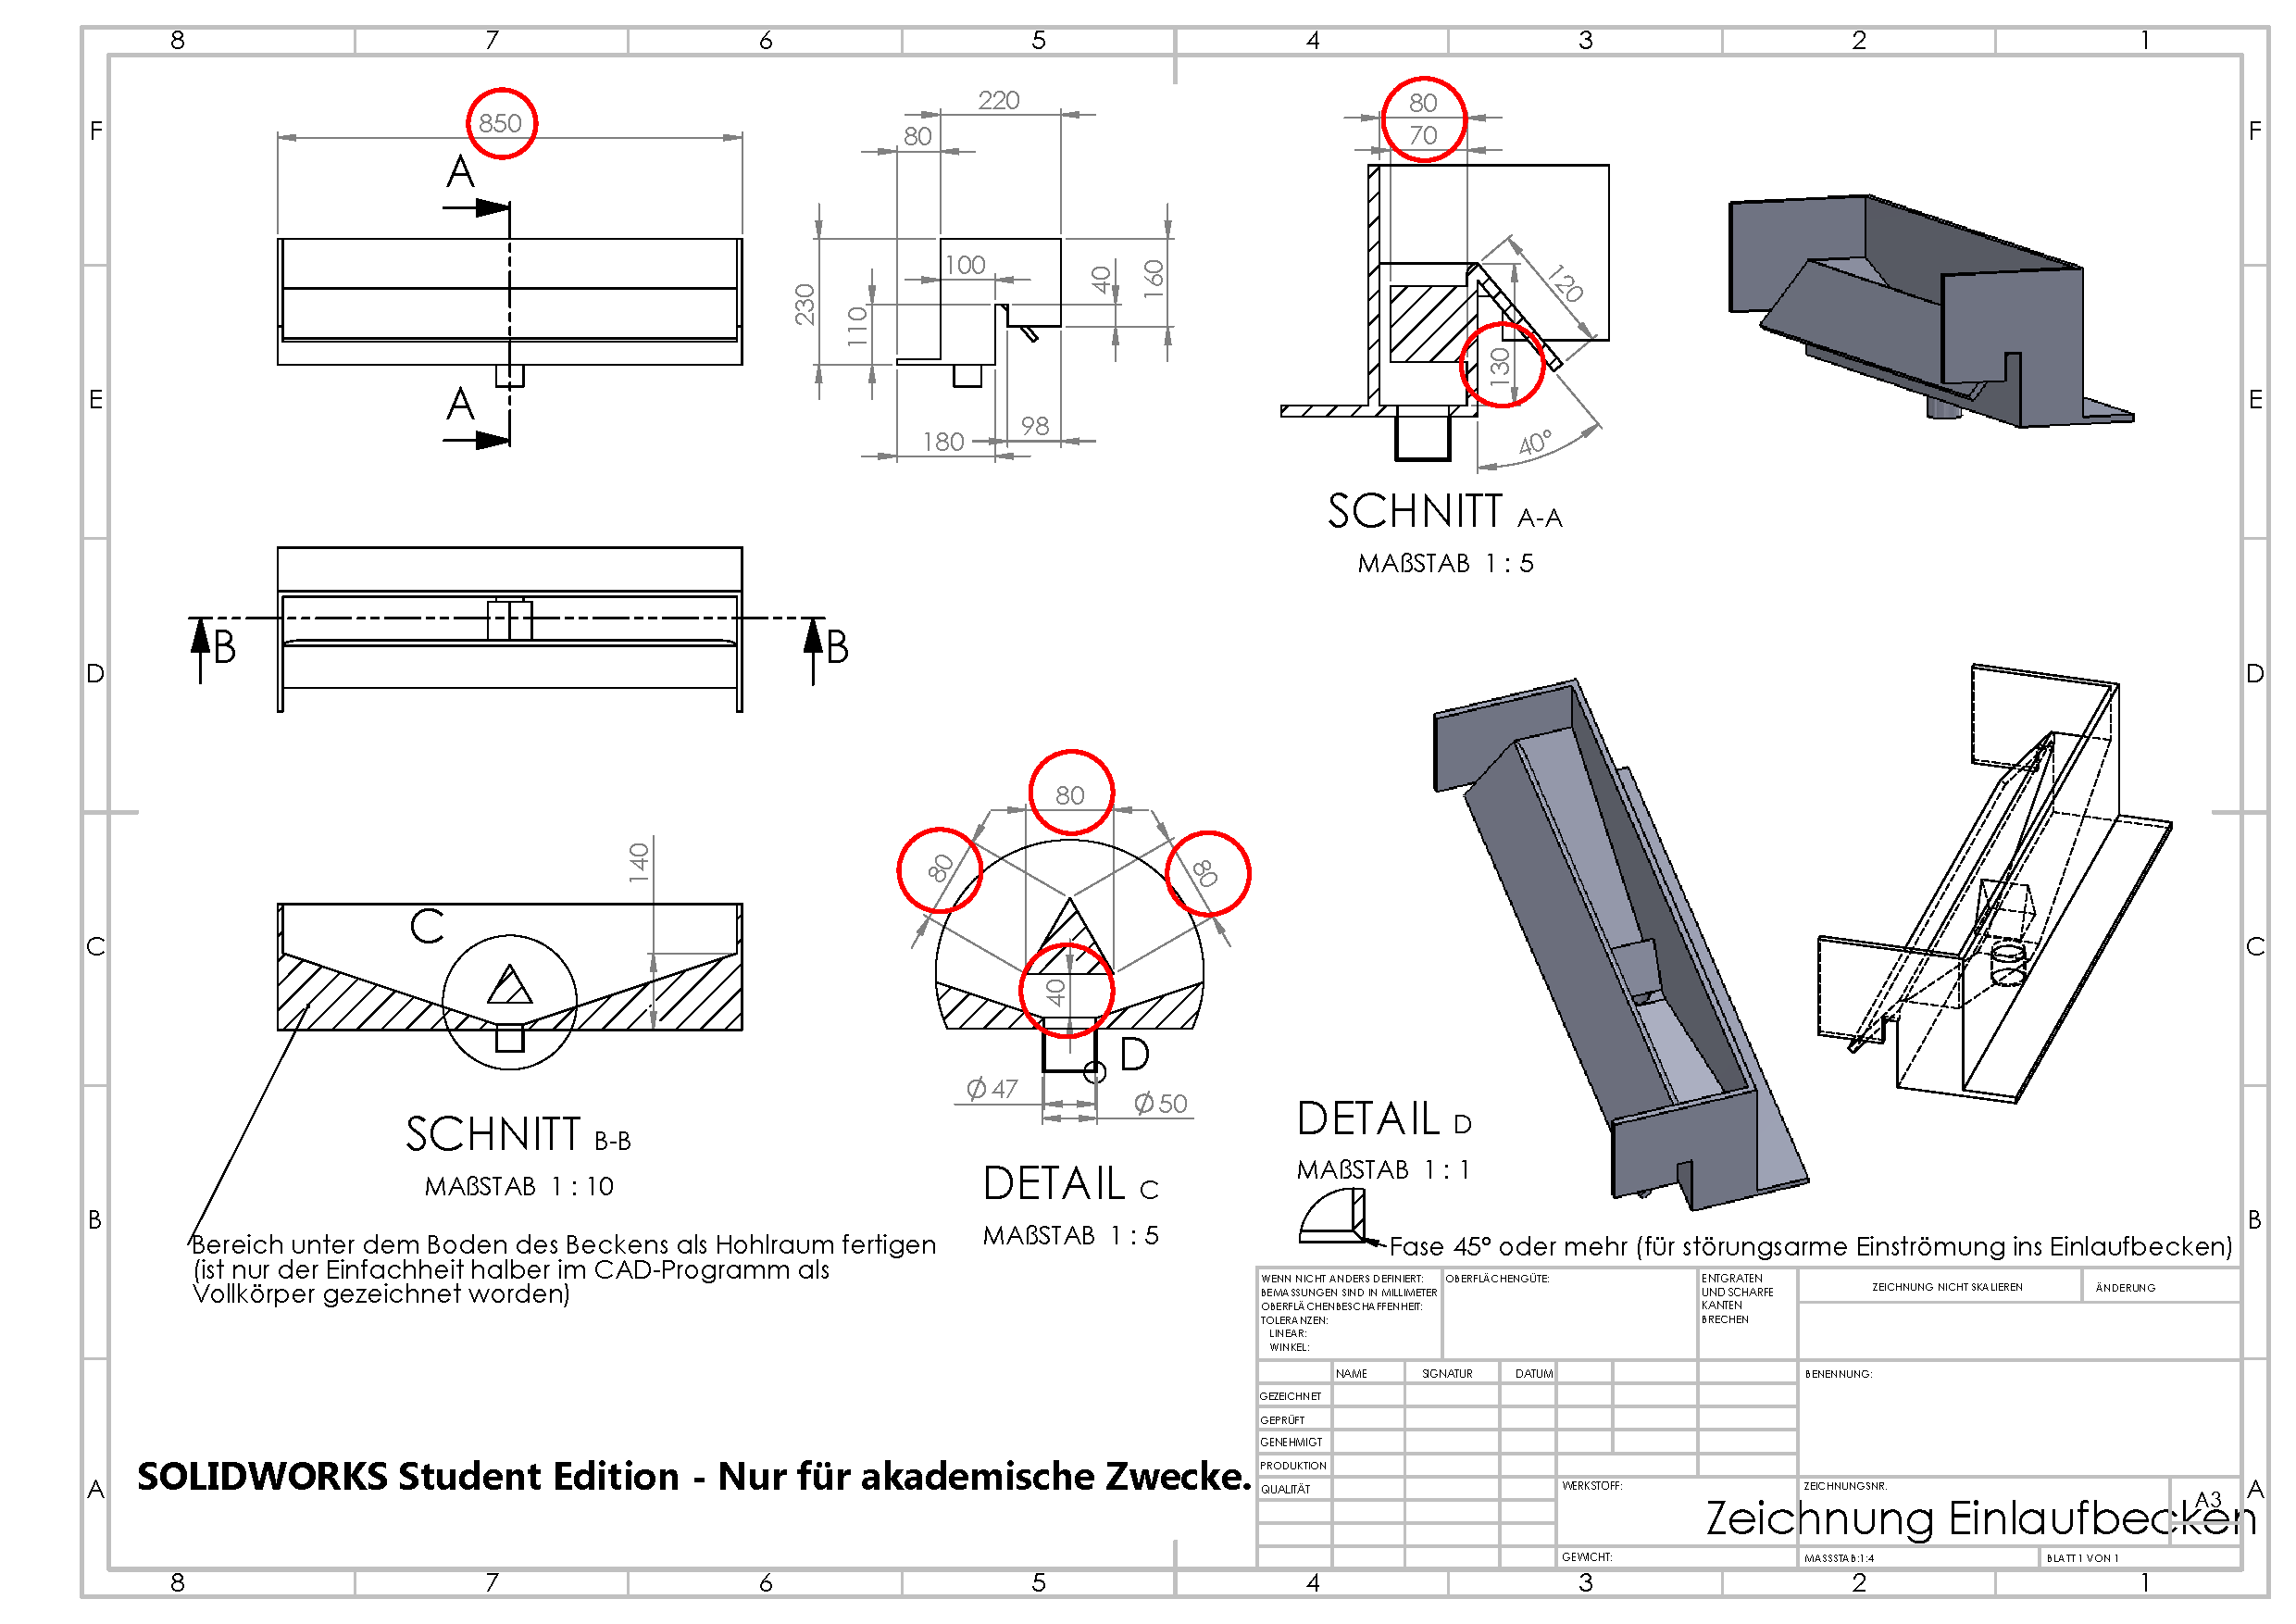
\includegraphics[width=\textwidth]{images/Einlaufbecken.pdf} 
		\caption{Forebay}
		\label{fig:elb}
	\end{center}
\end{figure}

\section{Electrical Conductivity Resolution}

To measure the arrival of the new water stream after switching the water feed, the system has to be able to distinguish between water with different salinity. The water used normally in the reactor is tap water with a salinity of about \unit[0.2]{\%}. The salinity of the added saltwater can be chosen freely. Water with a salinity of about \unit[5]{\%} is easily available in the facilities and offers a sensible choice. Assuming a reactor with \unit[65]{l} in circulation and an added saltwater impulse of \unit[5]{l}, the resulting salinity after perfect homogenization would be approximately \unit[0.5]{\%}. The system has to be able to clearly distinguish between all those salinities. The sensors sensitivity therefore shall be better than \unit[0.1]{\%} salinity.

\section{Cost}

The more sensors used, the more points in the stream can be measured and the better the image of the stream gets. Therefore, the cost per sensor has to be low enough to not be prohibitive of adding more sensors.
The cost of a high quality lab conductivity meter is in the range of \euro{1000} and was set as the goal of maximum cost for the sensor system. The number of sensors needed to cover all interesting regions of the bioreactors is about 40.
A cost per sensor of \euro{25} results from those figures.

\section{Usability}

The sensor system is meant to be used in the algae reactors of the algae cultivation center at the Ludwig Bölkow Campus. It has to be possible to easily mount and remove the system to and from the reactor without having to dismantle it.

The system also has to be easy to use, so it can be helpful to the researchers working on the reactor. It has to work reliably and act according to expectations of the users. The chance of handling errors that lead to loss of data has to be minimized. All operations have to be documented in a minimal set of written instructions, so the system can still be used even if the designer isn't available anymore.

\begin{table}[H]
    \centering

    \caption[Requirements]{Requirements}
    \label{tab:req}
    \begin{tabular}{lp{.7\textwidth}l}
        	\toprule
        	Nr. & Requirement & Verification \tabularnewline
        	\midrule
		1 & The system shall have a spacial resolution in the order of \unit[1]{cm}. & Inspection \tabularnewline
		2 & The system shall have a sensitivity of  \unit[0.1]{\%} salinity.  & Test \tabularnewline
		3 & The cost per sensor shall be less than \euro{25}.  & Analysis \tabularnewline
		4 & The system shall be deployable in the algae reactor. & Demonstr. \tabularnewline
		5 & The system shall be usable with a minimal set of written instructions. & Test, Review \tabularnewline
        \bottomrule
    \end{tabular}
\end{table}

\chapter{Background}

\section{Market Research}

Conductivity meters can be readily bought and range from prices of \euro{500} for lab equipment to \euro{10} for simple field water quality monitors. All available solutions are standalone devices using a single sensor and a display to report measurements. They also are designed to perform singular, high quality reads.

All of these traits are detrimental to the requirements of this project. A device is needed, which can perform fast measurements on multiple points in the stream, with the data exposed in a machine-readable format for further processing. Precision of the measurement can be compromised on, as long as a minimal standard is met. A custom design is necessary.

---
[stub. detailed description of electronics]
As base for this design, two solutions were found.
[mini-eC Interface]
Open Hardware implementation of simple signal generator and signal reader for a two electrode sensor providing raw voltage drop output.
[AD5933]
A simple signal generator and signal reader for a two electrode sensor, providing impedance with real and imaginary part. [this is the circuitry from the mini-eC-Interface on a single chip! awesome! base for version 2!]
---

\section{Theoretical Background}

[subsections?]

The conductivity $ \kappa $  is the ability of a substance to conduct electricity. It is measured in the unit \unitfrac{S}{m} and is a specific parameter normalized to length. To better understand conductivity, an equivalent circuit diagram \ref{fig:ecd} of the experiment design \ref{fig:elec} can be used. In this experiment, the resistance of a substance is determined by measuring the potential drop. [update figures with voltage divider]

The resistance is
\begin{equation}
	R = \dfrac{U}{I}
\label{eq:R}
\end{equation}

The inverse of $ R $ is the conductance
\begin{equation}
	G = \dfrac{I}{U}
\label{eq:G}
\end{equation}

Considering the cell constant $ C $ yields the conductivity
\begin{equation}
	\kappa = G \cdot \kappa
\label{eq:kappa} 
\end{equation}

The cell constant depends on the geometry of the sensor
\begin{equation}
	C = \dfrac{d}{A}
\label{eq:C}
\end{equation}

where $ d $ is the distance between and $ A $ the size of  the electrodes. [add figure of sensor geometry]

\begin{figure}
	\begin{center}
		\begin{circuitikz}[european voltages]
			\draw
  			(0,0) to [short, *-] (2,0)
  			to [R, l_=$R$] (2,4)
  			(0,0) to [open, v^<=$U$] (0,4)
  			to [short, *- ,i=$I$] (2,4);
		\end{circuitikz}
		\caption{equivalent circuit diagram}
		\label{fig:ecd}
	\end{center}
\end{figure}

\begin{figure}
	\begin{center}
    	\tikzset{external/export next=false}
		\begin{tikzpicture}
  		    % Draw electrode
 	   		\fill [black!25] (0.5,2) rectangle (1.5,-1);
	    		% draw voltmeter
 	   		\draw[join = round, thick] (1,2) -- (1,2.5) -- (2.4,2.5);
 	   		\draw[join = round, thick] (3.1,2.5) -- (4.5,2.5) -- (4.5,2);
 	   		\draw (2.75,2.5) node [circle, draw] {V};
  	  		%Draw electrode
  	  		\fill [black!25] (4,2) rectangle (5,-1);
    		%Draw water
    		\fill [blue!75, opacity=0.3] (-0.5,1) rectangle (6,-2);
		\end{tikzpicture}
		\caption{electrode configuration}
		\label{fig:elec}
	\end{center}
\end{figure}

[paragraphs with line inbetween?]
The principle of determining conductivity of a substance by measuring it's resistance in a defined geometry is called conductometry. In electrolytes, the electrical conduction happening is a result of mass transfer, where ions are carrying the charges. If the measurement is conducted with direct current, this mass transfer leads to changes in the measured solution and the electrode surface, negatively impacting the measurement. Furthermore, polarization effects create additional resistance, leading to lower than actual results. To avoid this, alternating current is used. The fast, periodical swap of polarity eliminates the net mass flow and it's effects. Polarization is a result of the current through the electrode, thereby it's effects can be minimized by minimizing this current.

The electrolytes temperature has a big influence on the conductivity and has to be taken in account when comparing two measurements. If the temperature is known, the conductivity can be normalized to a reference temperature.

The system described above is called a two-electrode-cell. In order to minimize current through the electrode, it is possible to separate the current flow from the potential measurement by using four electrodes. One pair is used to apply the current, a separate pair is used to measure the potential drop. This system is called a four-electrode-cell.

[everything up to here is translated and paraphrased from]
\cite{trankler2015sensortechnik}
[how do I make that clear?]


\chapter{Design}

This chapter describes the design of the sensor system and all components involved. The system consists of several parts playing different roles. The System Design gives an overview of these parts, their purpose and their communication with each other. Afterwards, these subsystem are described in detail.\\

\section{System Design}

On the user-facing side there is a personal computer (PC). This PC runs software that visualizes a live data stream and provides a control interface for the sensor system. It is connected via USB to a microcontroller. This microcontroller controls the MinieeC interface via I2C, reads the measurement data from it and sends it to the PC. It also controls the matrix switches. The MinieC Interface provides the signal and ground between which the resistance is measured. Both lines are connected to one matrix switch each. These matrix switches are able to connect one input to 8 different outputs. On each of those outputs, one electrode is connected. The matrix switches can thereby connect the MinieC interface to one of 8 electrode pairs. \\

Using the matrix switches, 8 electrodes can be used with just one MinieC interface. Increasing the number of electrodes can be done in two ways:

\begin{itemize}
    \item by chaining up multiple stages of matrix switches, the number of electrodes can be increased eightfold with each stage
    \item by connecting another MinieC Interface with it's own set of matrix switches to the microcontroller, 8 more electrodes can be added with each of these subsystems
\end{itemize}

The first option results in lower cost per added electrode, as the MinieC interface is reused. However, with a system like that, all electrodes have to be read in serial, while with the second option each MinieC interface can read in parallel, resulting in higher sample rate. Practically the second option is also easier to achieve. For the first option, a board with 18 matrix switches and 80 connections is needed, while the second option only uses 2 switches per board resulting in 16 connections. The simpler board greatly reduces complexity and can also be made smaller.

\begin{figure}
	\begin{center}
\begin{tikzpicture}
	\begin{pgfonlayer}{nodelayer}
		\node [rounded corners=8pt, inner sep=16pt, style=rect] (0) at (8, -1) {8 Electrodes};
		\node [rounded corners=8pt, inner sep=16pt, style=rect] (1) at (0, 3) {Microcontroller};
		\node [rounded corners=8pt, inner sep=16pt, style=rect] (2) at (-3, -1) {MinieC Interface};
		\node [rounded corners=8pt, inner sep=16pt, style=rect] (3) at (3, 0.25) {Matrix Switch};
		\node [rounded corners=8pt, inner sep=16pt, style=rect] (4) at (0, 6) {PC};
		\node [style=rect, inner sep=16pt, rounded corners=8pt] (5) at (3, -2.25) {Matrix Switch};
	\end{pgfonlayer}
	\begin{pgfonlayer}{edgelayer}
		\draw [style=darrow] (4) to node[left]{USB} (1);
		\draw [style=simple, bend right=15, looseness=1.00] (0) to node[above]{8 SIG} (3);
		\draw [style=simple, bend right=15, looseness=1.00] (3) to node[above]{SIG} (2);
		\draw [style=arrow, bend left=15, looseness=1.00] (1) to node[right]{SPI} (3);
		\draw [style=darrow, bend right=15, looseness=1.00] (1) to node[left]{I2C} (2);
		\draw [style=simple, bend right=15, looseness=1.00] (2) to node[below]{GND} (5);
		\draw [style=simple, bend right=15, looseness=1.00] (5) to node[below]{8 GND} (0);
		\draw [style=arrow, bend left=15, looseness=1.00] (1) to node[right, pos=0.9]{SPI} (5);
	\end{pgfonlayer}
		\draw (-5.5,-3.5) -- (10,-3.5) -- (10,2) node[below, left, yshift=-8pt] {$n$} -- (-5.5,2) -- (-5.5,-3.5);
\end{tikzpicture}
		%\begin{tikzpicture}
	\begin{pgfonlayer}{nodelayer}
		\node [rounded corners=8pt, inner sep=16pt, style=rect] (0) at (8, -1) {8 Electrodes};
		\node [rounded corners=8pt, inner sep=16pt, style=rect] (1) at (0, 3) {Microcontroller};
		\node [rounded corners=8pt, inner sep=16pt, style=rect] (2) at (-3, -1) {MinieC Interface};
		\node [rounded corners=8pt, inner sep=16pt, style=rect] (3) at (3, 0.25) {Matrix Switch};
		\node [rounded corners=8pt, inner sep=16pt, style=rect] (4) at (0, 6) {PC};
		\node [style=rect, inner sep=16pt, rounded corners=8pt] (5) at (3, -2.25) {Matrix Switch};
	\end{pgfonlayer}
	\begin{pgfonlayer}{edgelayer}
		\draw [style=darrow] (4) to node[left]{USB} (1);
		\draw [style=simple, bend right=15, looseness=1.00] (0) to node[above]{8 SIG} (3);
		\draw [style=simple, bend right=15, looseness=1.00] (3) to node[above]{SIG} (2);
		\draw [style=arrow, bend left=15, looseness=1.00] (1) to node[right]{SPI} (3);
		\draw [style=darrow, bend right=15, looseness=1.00] (1) to node[left]{I2C} (2);
		\draw [style=simple, bend right=15, looseness=1.00] (2) to node[below]{GND} (5);
		\draw [style=simple, bend right=15, looseness=1.00] (5) to node[below]{8 GND} (0);
		\draw [style=arrow, bend left=15, looseness=1.00] (1) to node[right, pos=0.9]{SPI} (5);
	\end{pgfonlayer}
\end{tikzpicture}
		%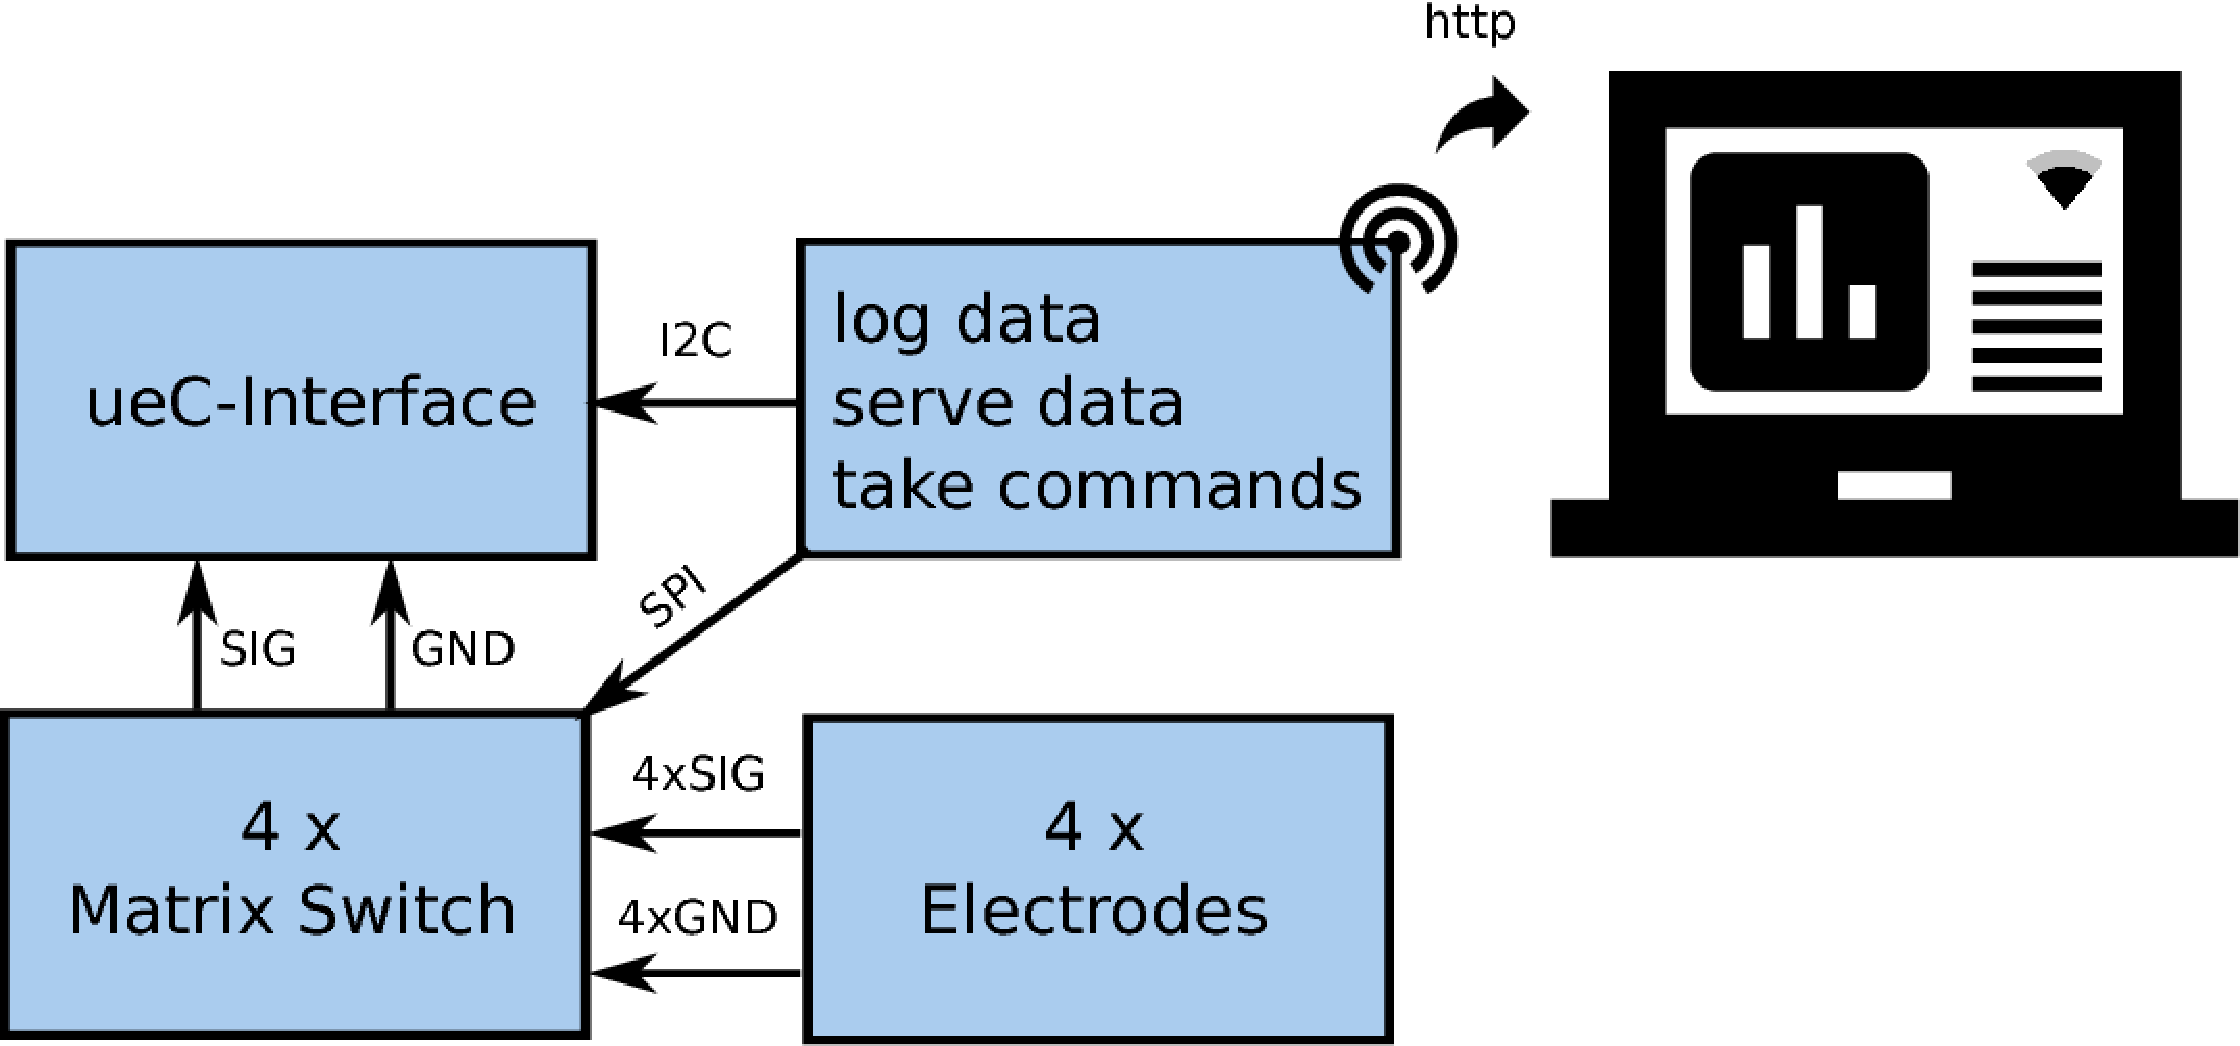
\includegraphics[width=\textwidth]{images/systemdesign.pdf} 
		\caption{System Design}
		\label{fig:sys}
	\end{center}
\end{figure}

\section{Electrodes}

The electrode pairs are the actual sensors in contact with the fluid to be measured. Their material and geometry influence the measuring range of the system. According to information in the book \cite{trankler2015sensortechnik} a cell constant $ C $ of $1$ enables a range from \unitfrac[$2 \cdot 10^3$]{$\mu S$}{cm} to \unitfrac[$10 \cdot 10^3$]{$\mu S$}{cm}. For a water temperature of \unit[$18^\circ$]{C} this corresponds to salinities of \unit[0.66]{\%} and \unit[0.12]{\%}. While this theoretical range is not sufficient for our purpose, first tests showed that the achievable range is much bigger than described in the book. The book doesn't specify the materials influence on the range and it also doesn't qualify how the usable range is defined. As our application has much lower demands on accuracy as the usual ones, this might be an explanation for the discrepancy. \\

Figure \ref{fig:sensor} shows the geometry of the sensor. To achieve a cell constant $C$ of $1$, a width $w$ of \unit[1]{mm}, height $h$ of \unit[10]{mm} and distance $d$ of \unit[10]{mm} were chosen.\\

\begin{figure}
	\begin{center}
		\begin{tikzpicture}
			\draw [line width=0.5mm] (-1,-1) -- (-1,1) -- (-1.3,1) -- (-1.3,-1) -- (-1,-1);
			\draw [dash dot] (-1.15,-1.5) -- (-1.15,1.2);
			\draw [line width=0.5mm] (1,-1) -- (1,1) -- (1.3,1) -- (1.3,-1) -- (1,-1);
			\draw [dash dot] (1.15,-1.5) -- (1.15,1.2);

			\draw (-1,1.6) -- (-1,1);
			\draw (-1.3,1.6) -- (-1.3,1);
			\draw (-1,1.4) -- (-1.3,1.4) node[above, pos=-0.75] {$w$};
			\draw [arrow]  (-1.7,1.4) -- (-1.3,1.4);
			\draw [arrow] (-0.6,1.4) -- (-1,1.4);
			
			\draw (-1.9,1) -- (-1.3,1);
			\draw (-1.9,-1) -- (-1.3,-1);
			\draw [darrow] (-1.7,1) -- (-1.7,-1) node[left, pos=0.5] {$h$};

			\draw [darrow] (-1.15,-1.3) -- (1.15,-1.3) node[above, pos=0.5] {$d$};

		\end{tikzpicture}
		\caption{Electrode pair forming a sensor}
		\label{fig:sensor}
	\end{center}
\end{figure}

As a first proof-of-concept a the sensor was built as a sensor array, containing multiple electrode pairs on a strip \ref{fig:v2}. A \unit[5]{cm} wide and \unit[25]{cm} long band of Kapton adhesive tape served as the base. 4 electrode pairs made from \unit[0.2]{mm} platinum wire were arranged equidistant on the strip. \unit[0.4]{mm} enameled copper wire runs along the tape to connect each electrode pair to the left end of the strip, from which insulated cables run to the sensor node. After soldering the joints, two smaller strips of tape were used to cover the wiring, exposing only the electrodes to fluid.

First tests with this sensor array showed the viability of the concept, however a simple look at it shows the inherit problems. Instead of a uniformly flat strip with minimal influence on the flow, the assembly forms several irregularities. Soldering \unit[0.2]{mm} platinum wire to \unit[0.4]{mm} enameled copper wire on a piece of adhesive tape per hand also did not result in clean solder joints. And while with the experience of the first array, the second array turned out a bit cleaner, the fundamental problem remains: it is a tedious manufacturing process resulting in a low quality product.

\begin{figure}
	\begin{center}
		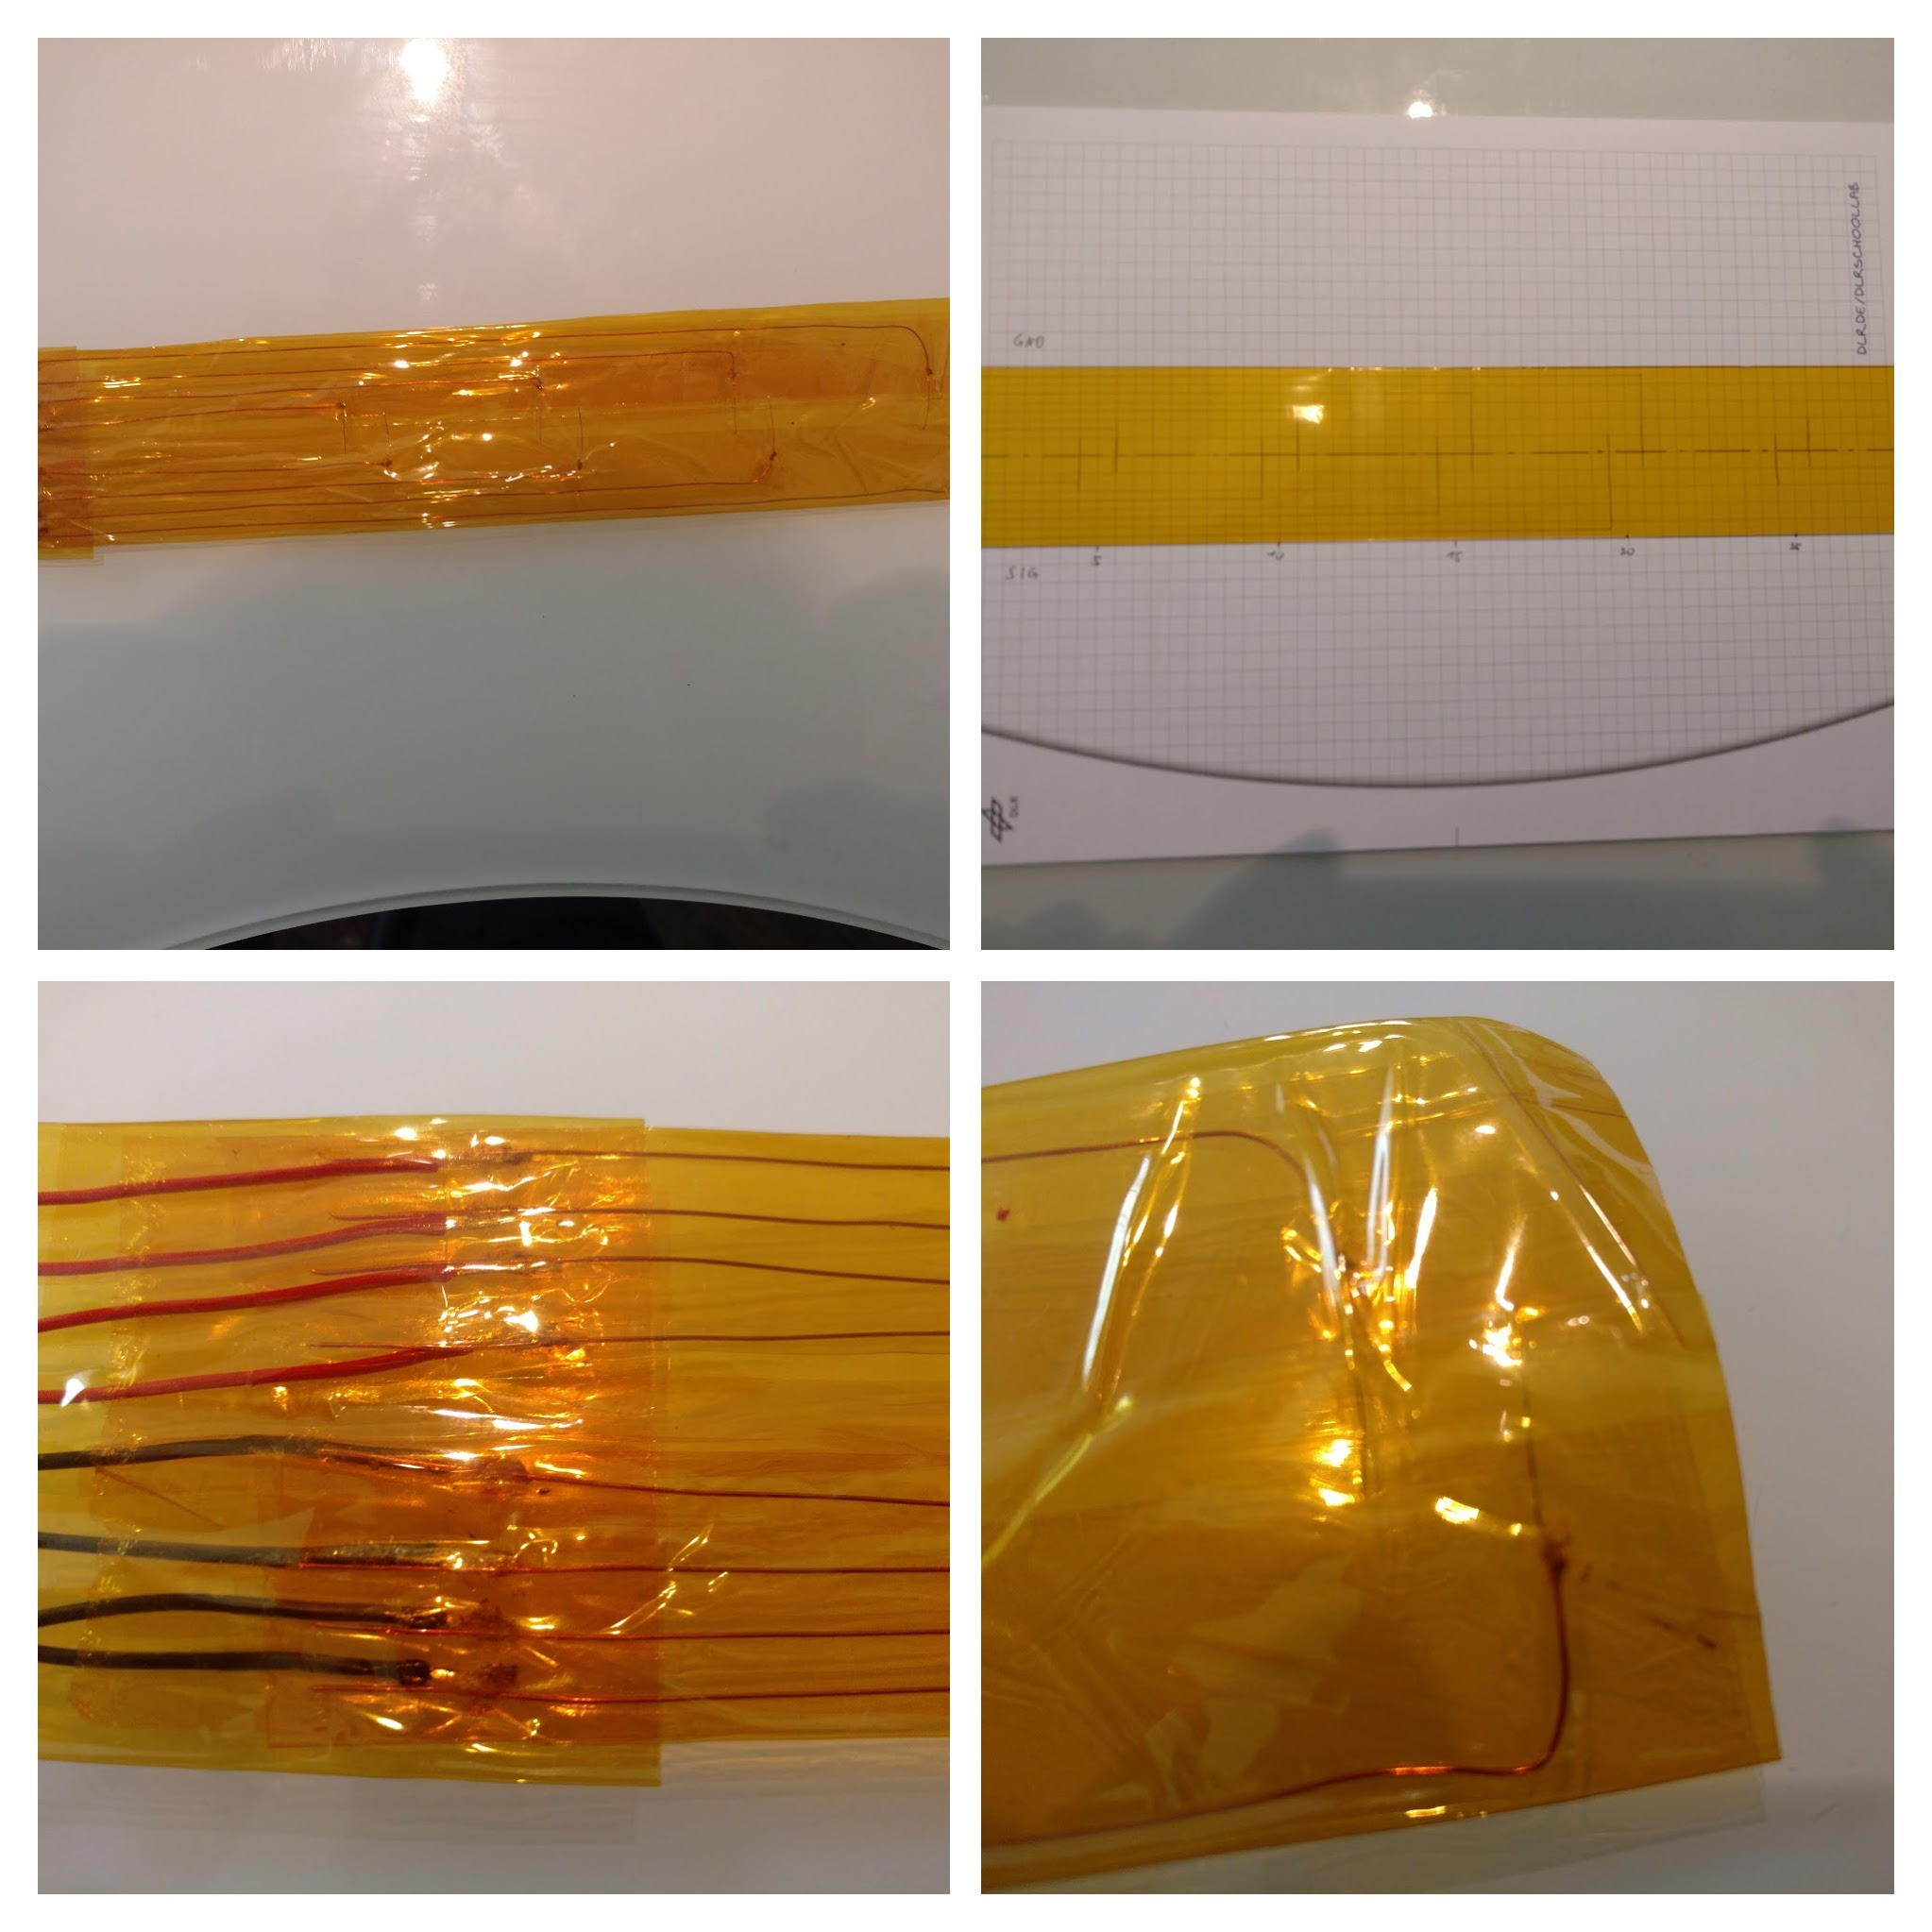
\includegraphics[width=\textwidth]{images/v2.jpg} 
		\caption{Handmade Sensor Strip}
		\label{fig:v2}
	\end{center}
\end{figure}

As an alternative to these handmade strips, industrially produced Flex-PCBs were identified. Flex-PCBs are flexible printed circuit boards that are very close to the handmade arrays described above. They also use Kapton as base, on which a copper coating gets applied and partially removed by etching to form the conducting paths. On top, another layer of Kapton is applied, with cutouts in the places where the copper is supposed to be exposed. The exposed copper is then plated with ENIG (Electroless nickel immersion gold) to protect the copper from oxidation and provide the landing pads for electrical components to be soldered on.

For our purpose those exposed and plated landing pads can be used as electrodes, being nicely embedded in a FlexPCB that also runs the wiring up to an interface from where cables can be run. Using the FlexPCB itself as cable is not viable due to the high cost per area.

The cables are soldered directly to the PCB and silicone is used to create a waterproof seal around the connection.

\begin{figure}
	\begin{center}
		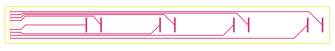
\includegraphics[width=\textwidth]{images/fpcbd.pdf} 
		\caption{Design of FlexPCB}
		\label{fig:fpcbd}
	\end{center}
\end{figure}

\section{Matrix Switches}

The matrix switches are an essential part of the system, enabling it use multiple sensors with a single MinieC Interface, thus lowering the cost per sensor. The part used is an ADG738 from Analog Devices. It is an 8-channel CMOS analog matrix switch controlled via a 3-wire serial interface. The following information is taken from the data sheet \cite{ms}.\\

Figure \ref{fig:ms} shows the functional block diagram. The switch has one drain pin (D) and 8 source pins (S1..S8). Despite the naming of drain and source, the internals provide simple switches between the drain and each source pin. The switches work in both directions without any restriction on the signal beyond a maximum current of \unit[120]{mA} that far exceeds our needs. By sending control commands via the 3-wire interface, each of the 8 internal switches can be turned on and off individually.\\

\begin{figure}
	\begin{center}
		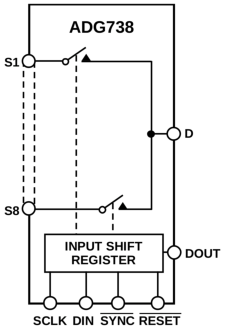
\includegraphics[width=0.3\textwidth]{images/ms.pdf} 
		\caption{Functional block diagram of ADG738}
		\label{fig:ms}
	\end{center}
\end{figure}

The example timing diagram \ref{fig:msc} describes the data transmission process. The microcontroller sends one byte of data to the matrix switch. Each of the 8 bits of this byte controls one switch. The first bit controls the first switch and so on. If the bit is 1, the switch is closed, if 0, the switch is open. To send the byte, first the synchronization pin (SYNC) has to be pulled low from it's usual high level. A clock signal is provided to the clock pin (SCLK). At each falling edge of the clock signal, the data input (DIN) is read - where high leads to a 1-bit and low to a zero-bit. After 8 cycles, SYNC is pulled high again marking the end of data transmission with a full byte transferred. After that, the switches immediately take their instructed states with switching times in the order of \unit[100]{ns}. In the example shown, the first switch is on, while all others are off.\\

\begin{figure}
	\begin{center}
	\tikzexternaldisable
		\begin{tikztimingtable}
  			SYNC   & H 32{L} H \\
  			SCLK   & C 16{2C} N(A1) C \\
  			DIN  	& 2{L} {2H} N(B1) 15{2L} \\
  			Data	& 2D{} 2D{1} 2D{} 2D{0} 2D{} 2D{0} 2D{} 2D{0} 2D{} 2D{0} 2D{} 2D{0} 2D{} 2D{0} 2D{} 2D{0} 2D{}\\
		\end{tikztimingtable}
		\caption{Timing diagram}
		\label{fig:msc}
	\end{center}
\end{figure}

Multiple matrix switches can be controlled at once by daisy-chaining the data output pin (DOUT) of the first device to DIN of the second one, and on so forth. Both SYNC and SCLK are connected to the same bus. This assures that all matrix switches are set in the same state and at the same time.

\section{MinieC Interface}

The sensor node logically consists of the signal generator and the signal reader, practically both parts are tightly integrated.

[Describe mini-eC-Interface]
[also where i.e. the change with the filter cap and the tests that surfaced the issue is described]

The mini-eC-Interface provides two channels to connect to the electrodes, but  multiple sensors should be driven by one interface. The method to this is called demultiplexing and the component able to this is the Matrix-Switch.
A Matrix-Switch is an electrical component containing a multitude of switches, where the switches can be electronically closed and opened from a controller. The Matrix-Switch chosen consists of 8 switches, where all switches have the same input, but separate outputs. Thus, they allow applying an input signal to different outputs. The input in our case is the signal and reference from the minie-eC-Interface, applied to 8 different electrode pairs making up the sensors. A separate Matrix-Switch is need for signal and reference.

\section{Microcontroller}

The Data Processing Unit has to be able to control the functions of the sensor nodes attached to it, read the data from them, log it and serve it to the user-interface. Typically, any micro-controller is is fit for those tasks. Micro-controllers usually are programmed in C or C++, however nowadays there are other options, too. One of those is Micropython, which is an implementation of the Python 3 programming language designed to run on micro-controllers. Python is a vastly easier language than C/C++, and this is especially true when the involved persons are not from a computer science or electrical engineering background, but i.e. mechanical engineering or other sciences. In those fields, Python is often familiar from usage for data processing and visualization. Using Micropython enables us to design a system where it is more likely that the people using it are able to understand the code, enabling them to improve it and adapt it to alternate use-cases.
It does however limit our choice of Hardware to supported platforms and it requires more powerful and thereby expensive micro-controllers. But as the system only requires one Data Processing unit to drive a very large amount of sensors, the added cost is relative and outweighed by the benefits of the better usability. While the factor of the expensive controllers to cheaper ones is about 10, the cost in the end is still only about \euro{7}.
For prototyping, a development board named "Espruino Pico" was chosen. It is a very small and simple board that provides the electrical boilerplate to use a micro-controller without needing to deal with the lowest level of electronics, like cleaning power supply, etc.

\section{User-Interface}
\chapter{Results}

In this chapter the verification and validation of the developed sensor system are described. The verification is a set of tests designed to review whether or not the system meets the requirements specified in the Chapter \ref{obj} Objectives. The validation is done by analyzing the data gathered during a number of experiments in the bioreactor.

\section{Verification}

\subsection{Spacial Resolution}

Requirement: The system shall have a spacial resolution in the order of \unit[10]{mm}.\\

An inspection of the physical size of the sensor and their placement on the array, drawn in Figure \ref{fig:sensarray}, shows us a sensor size of \unit[10x11]{mm} arranged on a grid of \unit[25x50]{mm}. The theoretical minimal grid size achievable with the chosen sensor size and a minimum distance between electrodes of \unit[1]{mm} is \unit[11x12]{mm}.
This grid size is the physical limitation of the spacial resolution and by being well within the order of \unit[10]{mm} meets the requirement.\\

\begin{figure}[H]
	\begin{center}
		\begin{tikzpicture}
		\begin{scope}
		\begin{scope}
			\draw [line width=0.5mm] (10,2.5) -- (-3,2.5) -- (-3,-2.5) -- (10,-2.5);
			\draw (10,2.5) .. controls (11,2) and (9,-2) .. (10,-2.5);
			\draw [dash dot] (-3.5,0) -- (11.5,0);
			\draw [darrow] (11,0) -- (11,-5) node[left, pos=0.45, xshift=-8pt, rotate=90] {25};
		
			\draw [line width=0.5mm] (-1,-1) -- (-1,1) -- (-1.3,1) -- (-1.3,-1) -- (-1,-1);
			\draw [dash dot] (-1.15,-1.5) -- (-1.15,1.2);
			\draw [line width=0.5mm] (1,-1) -- (1,1) -- (1.3,1) -- (1.3,-1) -- (1,-1);
			\draw [dash dot] (1.15,-1.5) -- (1.15,1.2);

			\draw (-1,1.6) -- (-1,1);
			\draw (-1.3,1.6) -- (-1.3,1);
			\draw (-1,1.4) -- (-1.3,1.4) node[above, pos=-0.75] {1};
			\draw [arrow]  (-1.7,1.4) -- (-1.3,1.4);
			\draw [arrow] (-0.6,1.4) -- (-1,1.4);
			
			\draw (-1.9,1) -- (-1.3,1);
			\draw (-1.9,-1) -- (-1.3,-1);
			\draw [darrow] (-1.7,1) -- (-1.7,-1) node[left, pos=0.2, xshift=-8pt, rotate=90] {10};

			\draw [darrow] (-1.15,-1.3) -- (1.15,-1.3) node[below, pos=0.5] {10};
			
			\draw [dash dot] (0,1.6) -- (0,-1.2);
			
			\draw [darrow] (0,1.4) -- (8,1.4) node[above, pos=0.5] {50};
		\end{scope}
		\begin{scope}[shift={(8,0)}]
			\draw [line width=0.5mm] (-1,-1) -- (-1,1) -- (-1.3,1) -- (-1.3,-1) -- (-1,-1);
			\draw [line width=0.5mm] (1,-1) -- (1,1) -- (1.3,1) -- (1.3,-1) -- (1,-1);
			\draw [dash dot] (0,1.6) -- (0,-1.2);
		\end{scope}
		\end{scope}
		\begin{scope}[shift={(0,-5)}]
		\begin{scope}
			\draw [line width=0.5mm] (10,2.5) -- (-3,2.5) -- (-3,-2.5) -- (10,-2.5);
			\draw (10,2.5) .. controls (11,2) and (9,-2) .. (10,-2.5);
			\draw [dash dot] (-3.5,0) -- (11.5,0);
			\draw [line width=0.5mm] (-1,-1) -- (-1,1) -- (-1.3,1) -- (-1.3,-1) -- (-1,-1);
			\draw [line width=0.5mm] (1,-1) -- (1,1) -- (1.3,1) -- (1.3,-1) -- (1,-1);
		\end{scope}
		\begin{scope}[shift={(8,0)}]
			\draw [line width=0.5mm] (-1,-1) -- (-1,1) -- (-1.3,1) -- (-1.3,-1) -- (-1,-1);
			\draw [line width=0.5mm] (1,-1) -- (1,1) -- (1.3,1) -- (1.3,-1) -- (1,-1);
		\end{scope}
		\end{scope}
		\end{tikzpicture}
		\caption{A dimensioned drawing of the sensor grid made up by two strips placed next to each other, not drawn to scale and cut on the right side. It shows the sensor size of \unit[10x11]{mm}, the horizontal distance between sensors of \unit[50]{mm} and the vertical distance of \unit[25]{mm}.}
		\label{fig:sensarray}
	\end{center}
\end{figure}

Due to the coupling of the spacial and time resolutions via the streams velocity as shown in Equation \eqref{eq:resv2}, this however is not sufficient to verify the requirement. 

\begin{equation}
	v = \dfrac{\diff s}{\diff t}
\label{eq:resv2} 
\end{equation}

A spacial resolution of \unit[10]{mm} would require a time resolution of \unit[0.01]{s}. However, this assumes the size $ l $ of the sensor and the time $ \tau $ a measurement takes to be infinitesimal small, which in reality it is not. While the sensors measures, the flow continuous and instead of measuring the conductivity of a certain volume at a certain time, an average is measured. Figure \ref{fig:cv} visualizes this issue.

\begin{figure}
	\begin{center}
		\begin{tikzpicture}
		\node [minimum height=32pt, minimum width=32pt, style=rect, fill opacity=0.2] (0) at (0, 0) {};
		\draw (-0.55,0) -- (-0.55,-1.5);
		\draw (0.55,0) -- (0.55,-1.5);
		\draw [darrow] (-0.55,-1.3) -- (0.55,-1.3) node[above, pos=0.5] {$l$};

		\node [minimum height=32pt, minimum width=32pt, style=vol] (0) at (-1.5, 0) {};
		\draw [arrow] (-2.05,1) -- (-1,1) node[above, pos=0.5] {$v$};
		\node [minimum height=32pt, minimum width=32pt, style=volb] (0) at (-2.6, 0) {};

		\node [] at (4,0) {$t<0$};

		\node [minimum height=32pt, minimum width=32pt, style=vol] (0) at (0, -2.5) {};
		\node [minimum height=32pt, minimum width=32pt, style=volb] (0) at (-1.1, -2.5) {};
		\node [minimum height=32pt, minimum width=32pt, style=rect, fill opacity=0.2] (0) at (0, -2.5) {};

		\node [] at (4,-2.5) {$t=0$};

		\node [minimum height=32pt, minimum width=32pt, style=vol] (0) at (0.25, -4) {};
		\node [minimum height=32pt, minimum width=32pt, style=volb] (0) at (-0.85, -4) {};
		\node [minimum height=32pt, minimum width=32pt, style=rect, fill opacity=0.2] (0) at (0, -4) {};

		\node [] at (4,-4) {$t=\tau$};		
		
		\node [minimum height=32pt, minimum width=32pt, style=vol] (0) at (1.5, -6) {};
		\node [minimum height=32pt, minimum width=32pt, style=volb] (0) at (0.35, -6) {};
		\node [minimum height=32pt, minimum width=32pt, style=rect, fill opacity=0.2] (0) at (0, -6) {};
				
		\node [] at (4,-6) {$t>\tau$};
		\end{tikzpicture}
		%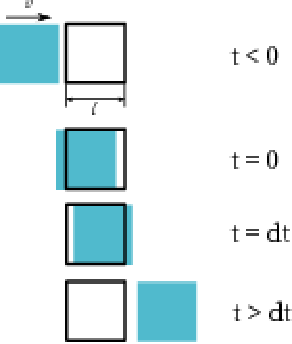
\includegraphics[width=0.45\textwidth]{images/resolution.pdf} 
		\caption{The control volumes in blue have the same size as the sensor (black rectangle). At $t=0$ the measurement starts and the first control volume is directly over the sensor. When  the measurement ends at $t=\tau$ the control volumes have moved. The sensor is covered by a mix of the two volumes.}
		\label{fig:cv}
	\end{center}
\end{figure}

To accommodate for that, factors $ n $ \eqref{eq:resn} and $ k $ \eqref{eq:resk} are introduced, describing the ratio of the resolutions to the actual sizes.

\begin{equation}
	n = \dfrac{l}{\diff s}
\label{eq:resn} 
\end{equation}

\begin{equation}
	k = \dfrac{ \tau}{\diff t}
\label{eq:resk}
\end{equation}

Inserting $ k $ and $ n $ in Equation \eqref{eq:resv} yields:

\begin{equation}
	v = \dfrac{\diff s}{\diff t} = \dfrac{k \cdot l}{n \cdot \tau}
\label{eq:resv1} 
\end{equation}

The ratio $ r $
\begin{equation}
	r = \frac{k}{n}
\label{eq:resr} 
\end{equation}
is the ratio of the time it takes a control volume to enter and leave the sensor area  to the time a measurement takes. Its inverse is the movement of the control volume during the measurement time and thereby the percentage by which the measured volume is bigger than the control volume. A ratio of 1 on would mean the measured volume is two times the sensor size, thereby halving the spacial resolution. To keep the resolution close the the sensor size, a ratio of 4, increasing the measured volume by \unit[25]{\%} is viable.
With the given sensor size and flow speed, a measurement time $ \tau $ of \unit[0.0025]{s} or \unit[2.5]{ms} is needed.\\

To test if the time resolution matches this, the measurement time itself can be timed. The difference between two adjacent times, i.e. the first time (\unit[975209221]{ns}) and the second time (\unit[975209961]{ns}), in the data set in Listing \ref{lst:data} is the measurement time of \unit[740]{ns}. The mean of the differences through the whole data set is \unit[748]{ns}. This means that the measurement is more than three times faster than required, showing that the time resolution easily matches the spacial resolution.

\begin{lstlisting}[caption={An excerpt of measurement data showing three lines of data from eight sensors. The long numbers are the times at which the measurements were taken in nanoseconds measured from the start, the short numbers are the measured values.},label={lst:data}]
975209221 21 975209961 59 975210676 15 975211397 0 975212119 0 975212840 26 975213554 59 975214276 9 
975215877 57 975216602 42 975217324 0 975218046 0 975218761 0 975219482 61 975220204 43 975220919 0 
975222520 52 975223271 0 975223993 0 975224708 0 975225429 45 975226150 53 975226867 0 975227583 0  
\end{lstlisting}

\subsection{Electrical Conductivity Resolution and Range}

Requirement: The system shall have a sensitivity of  \unit[0.1]{\%} salinity.\\
Requirement: The system shall have a range from 0 to \unit[5]{\%} salinity.\\

Table \ref{tab:rns} shows the results of measurements of solutions with different salinities. A \unit[10]{\%} solution was created by adding \unit[5]{g} of salt to \unit[100]{ml} of demineralized water. The subsequent solutions resulted from diluting the original one by adding more water.

The measurable change of the voltage was visible at the drop from a salinity of \unit[5]{\%} to \unit[2.5]{\%}. Between \unit[10]{\%} and \unit[5]{\%} no difference was measurable at all. The upper range limit can therefore be placed between \unit[5]{\%} and \unit[2.5]{\%}, above those values the sensor is saturated, providing only the information that the salinity is above the threshold.

On the lower limit, a measurement without any water, resulted in a voltage of \unit[0.02]{V}. This has to be considered the level of noise in the system. Above that, a clear distinction between salinities of \unit[0.08]{\%} and \unit[0.16]{\%} can be seen.

\begin{table}[H]
    \centering

    \caption[cal]{Range and Sensitivity}
    \label{tab:rns}
    \begin{tabular}{rr}
        	\toprule
        	Salinity in [\%] & Voltage in [V] \tabularnewline
        	\midrule
		10.00 & 0.95 \tabularnewline
        	5.00 & 0.95 \tabularnewline
		2.50 & 0.85 \tabularnewline
		1.25 & 0.65 \tabularnewline
		0.63 & 0.45 \tabularnewline
		0.31 & 0.28 \tabularnewline
		0.16 & 0.18 \tabularnewline
		0.08 & 0.11 \tabularnewline
		Air & 0.02 \tabularnewline
        \bottomrule
    \end{tabular}
\end{table}

While the requirement for sensitivity is clearly met, the range is just barely acceptable.

\subsection{Cost}

Requirement: The cost per sensor shall be less than \euro{25}\\

Using the bill of materials in Chapter \ref{BOM} a total price of \euro{121.8} for all materials for a sensor system with eight sensors can be calculated, resulting in a price per sensor of \euro{15.23}. Adding additional sensors after that would cost \euro{11.17} per sensor, as parts like the microcontroller do not have to be duplicated.

This price does not include the host PC as the PCs already installed in the laboratory can be used, as well as personal laptops like it was done in the testing phase. The demands on the host PC are very low, so in the worst case even a single board computer like the Raspberry Pie or similar can be used.

\subsection{Deployability in the Bioreactor}

Requirement: The system shall be deployable in the algae reactor.\\

The deployability was demonstrated during two test campaigns on the reactor. Figures \ref{fig:stripsr} and \ref{fig:pcr} show the set up during the tests. The host PC can be placed on a desk beside the reactor and connected to the carrier board with a USB cable. The carrier board can also be placed on desk or temporarily mounted on the reactor. The sensor strips connect to the carrier board with \unit[1]{m} long cables and are attached to the reactor with electrical tape.

\begin{figure}[H]
	\begin{center}
		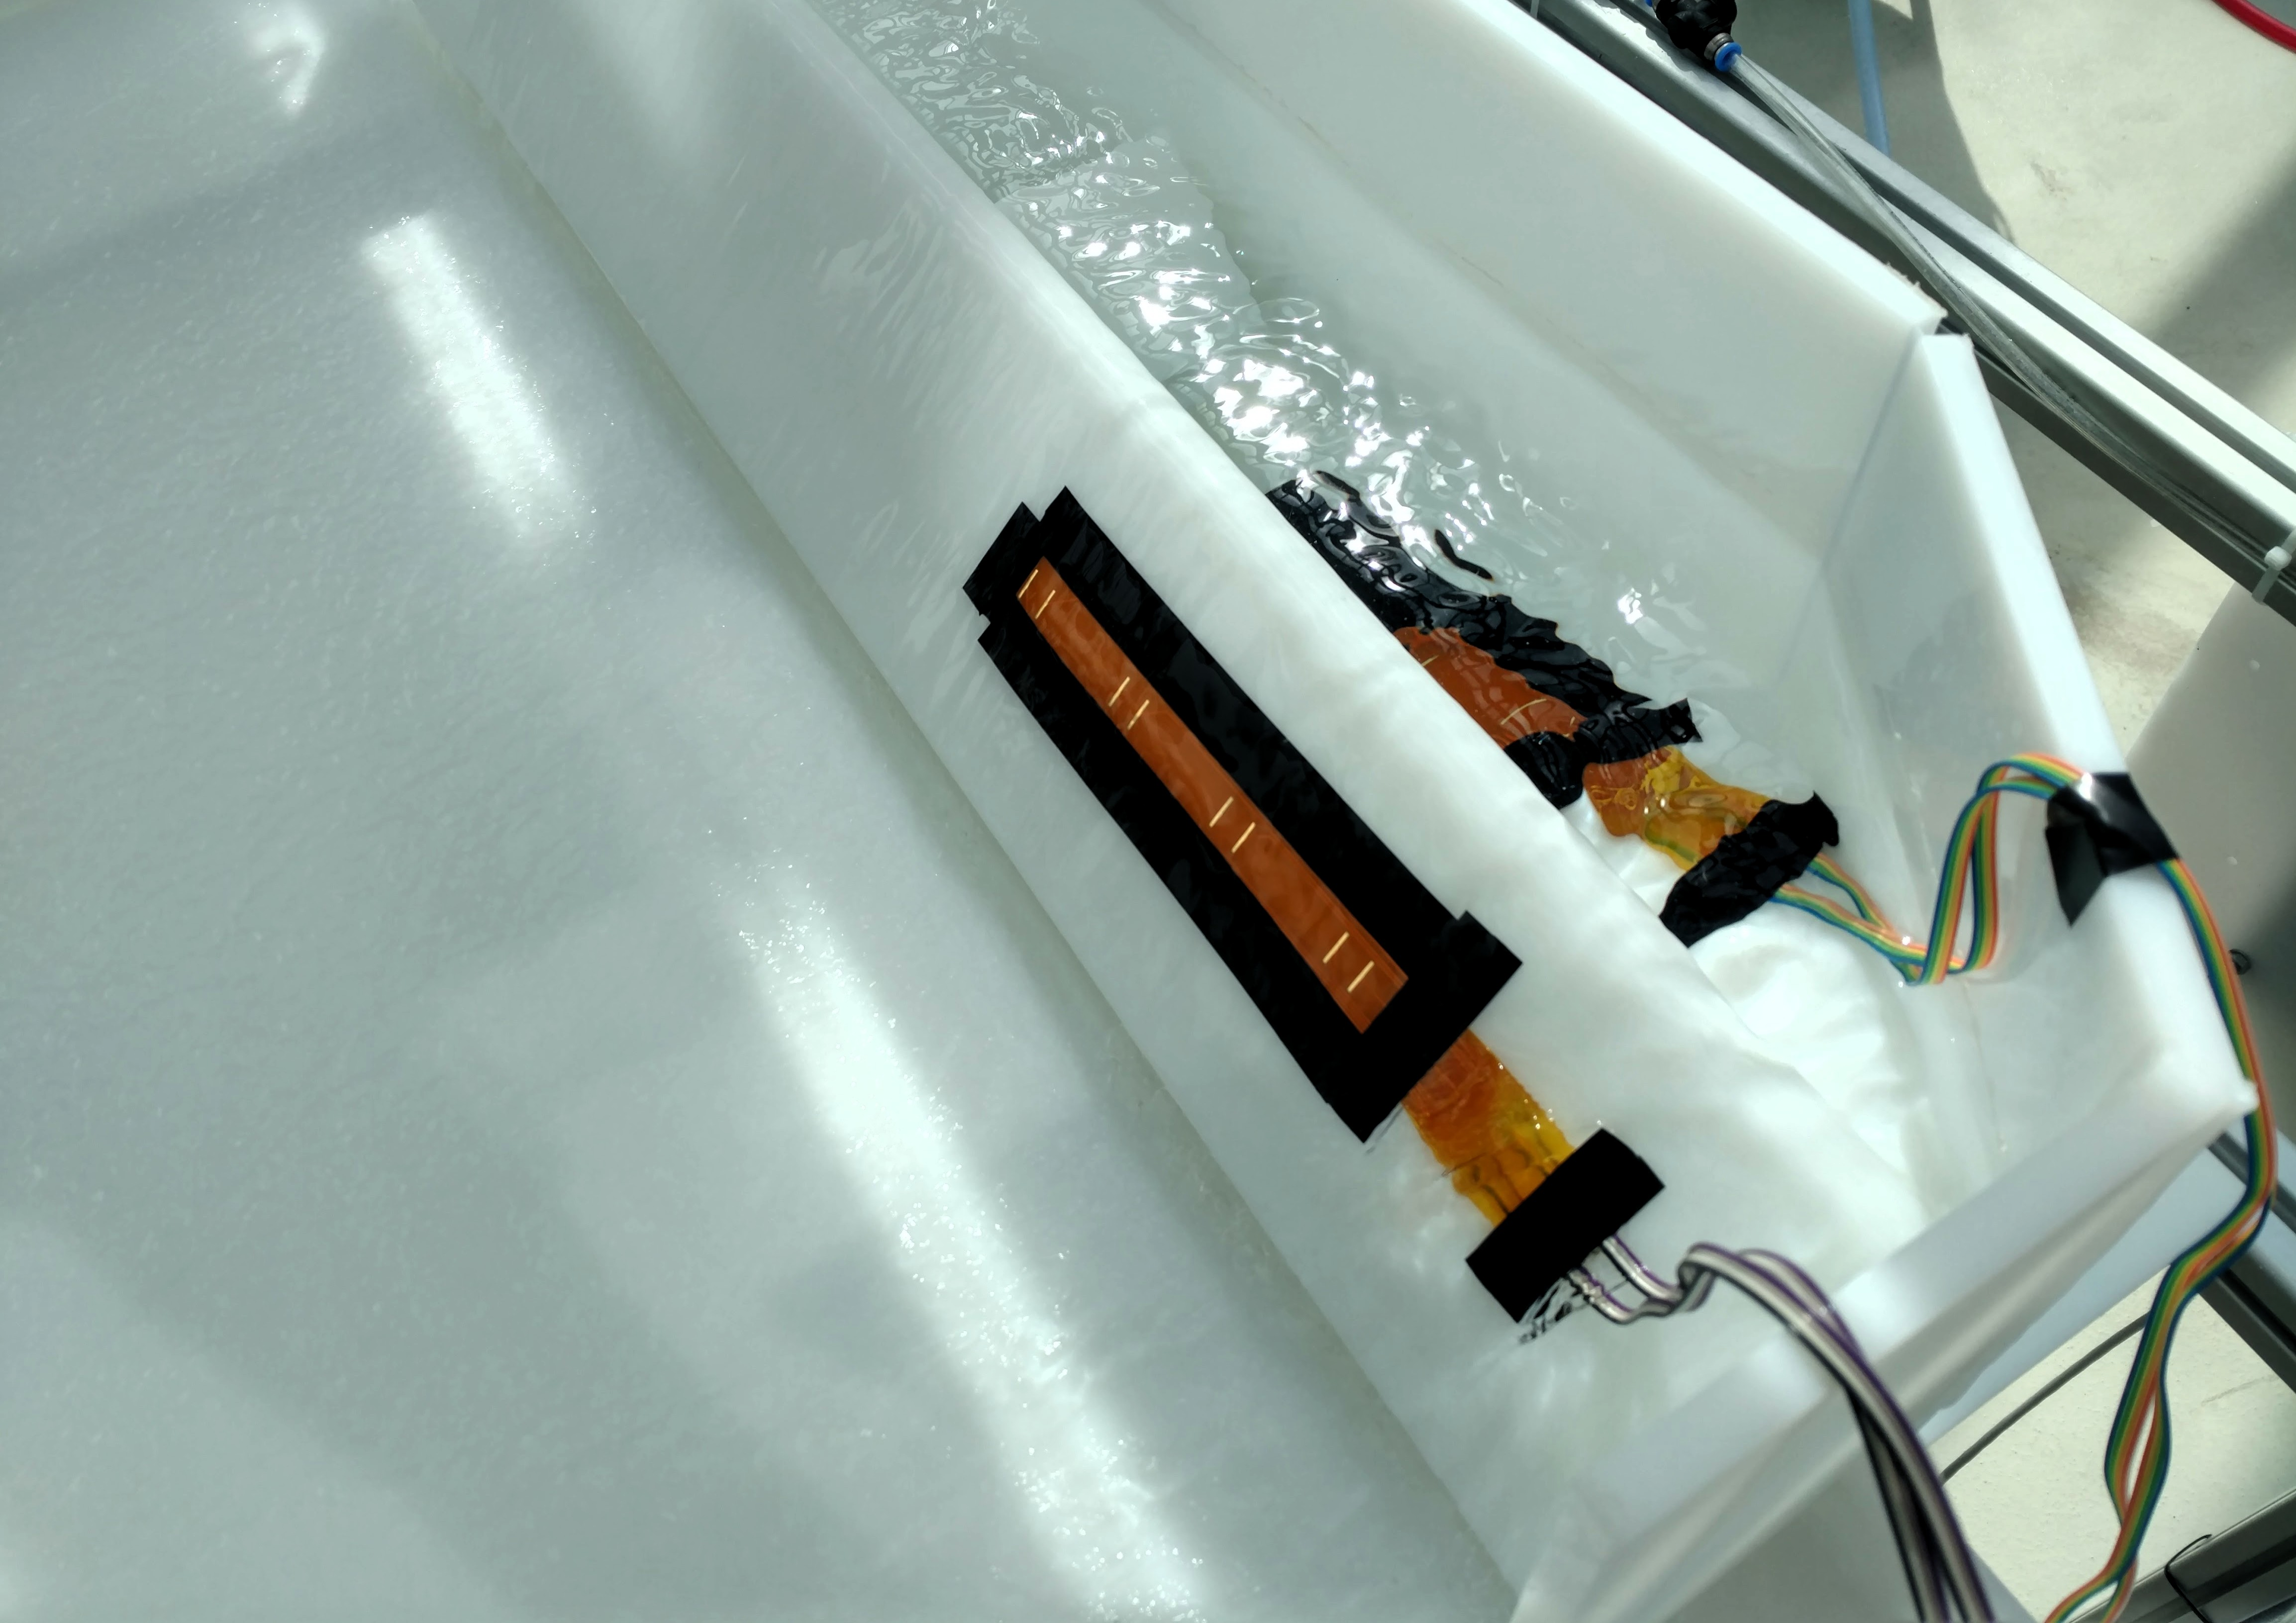
\includegraphics[width=0.8\textwidth]{images/stripsinreactor.jpg} 
		\caption{The sensor strips are mounted to the bioreactor with electrical tape. Cables of \unit[1]{m} length run towards the carrier board which is not in the frame.}
	\label{fig:stripsr}
	\end{center}
\end{figure}

\begin{figure}[H]
	\begin{center}
		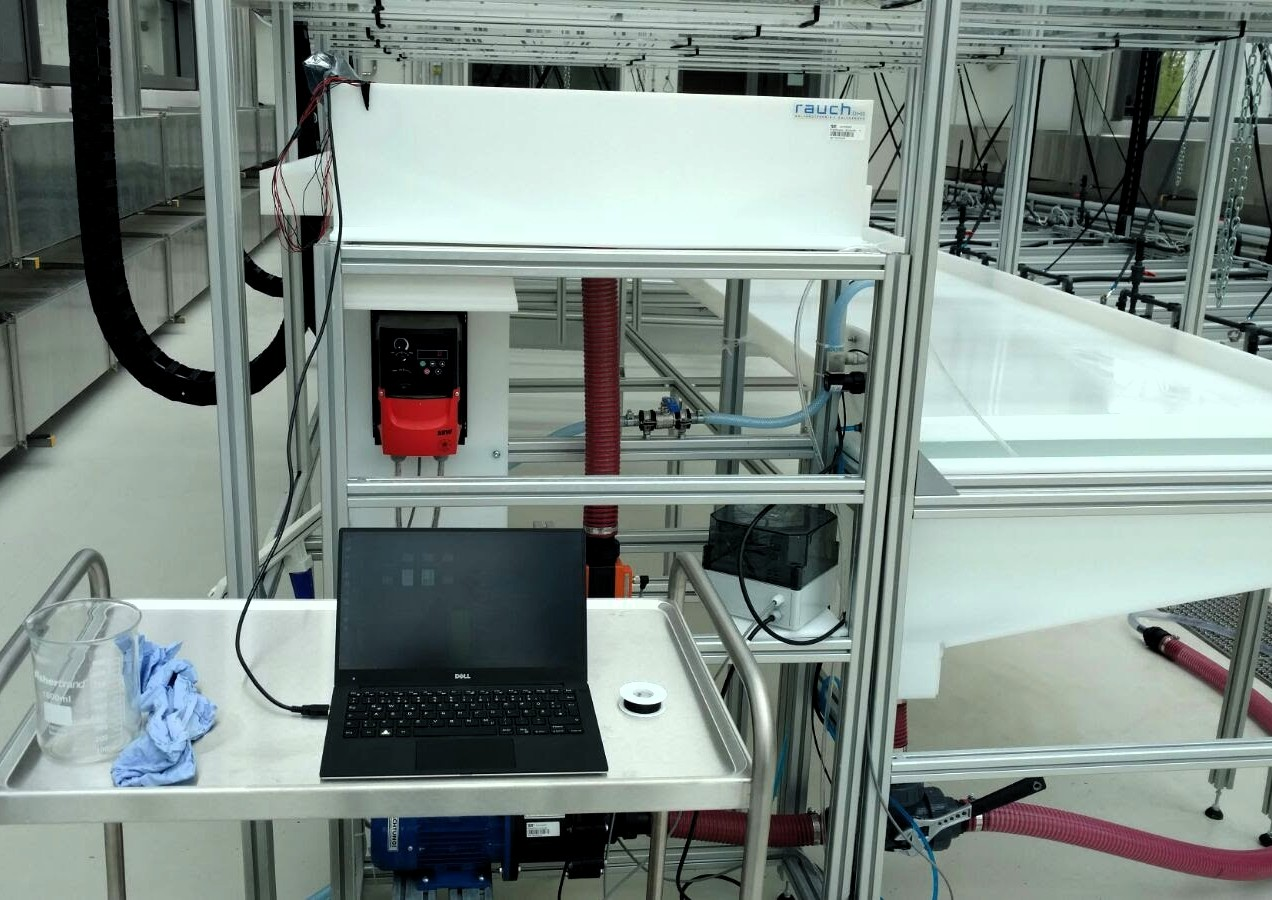
\includegraphics[width=0.8\textwidth]{images/pconreactor.jpg} 
		\caption{A laptop is used as host PC. A USB cable connects to the microcontroller on the carrier board, which is mounted on the side of the inlet basin.}
	\label{fig:pcr}
	\end{center}
\end{figure}

\subsection{Usability}

Requirement: The system shall be usable with a minimal set of written instructions.

The instructions for taking a series of measurements can be found in the Appendix. First, an image describes the different parts of the system relevant to the user. After that a step-by-step description with images helps the user through the process. All in all, only 8 steps are necessary.

\section{Validation} \label{val}

\begin{figure}
	\begin{center}
		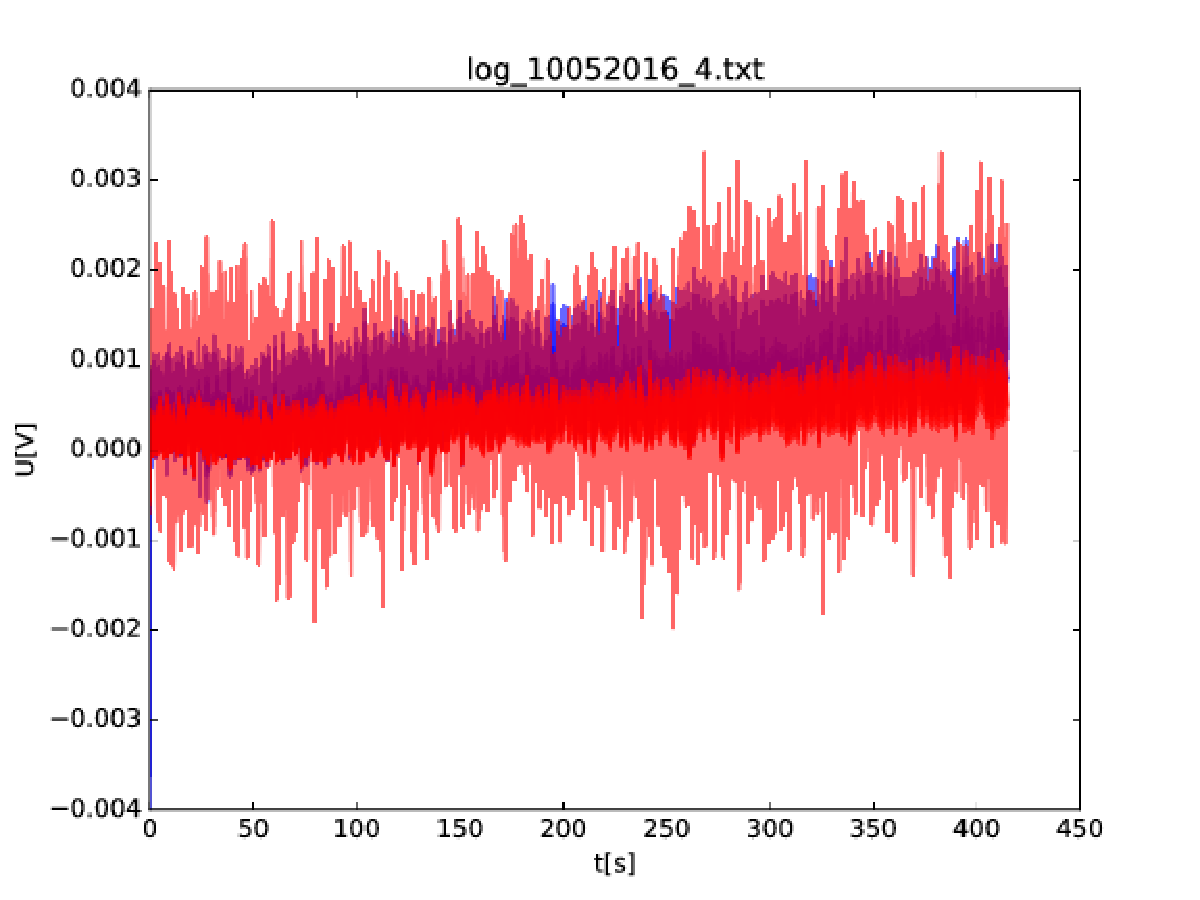
\includegraphics[width=\textwidth]{images/noise.pdf} 
		\caption{noise}
	\end{center}
\end{figure}

\begin{figure}
	\begin{center}
		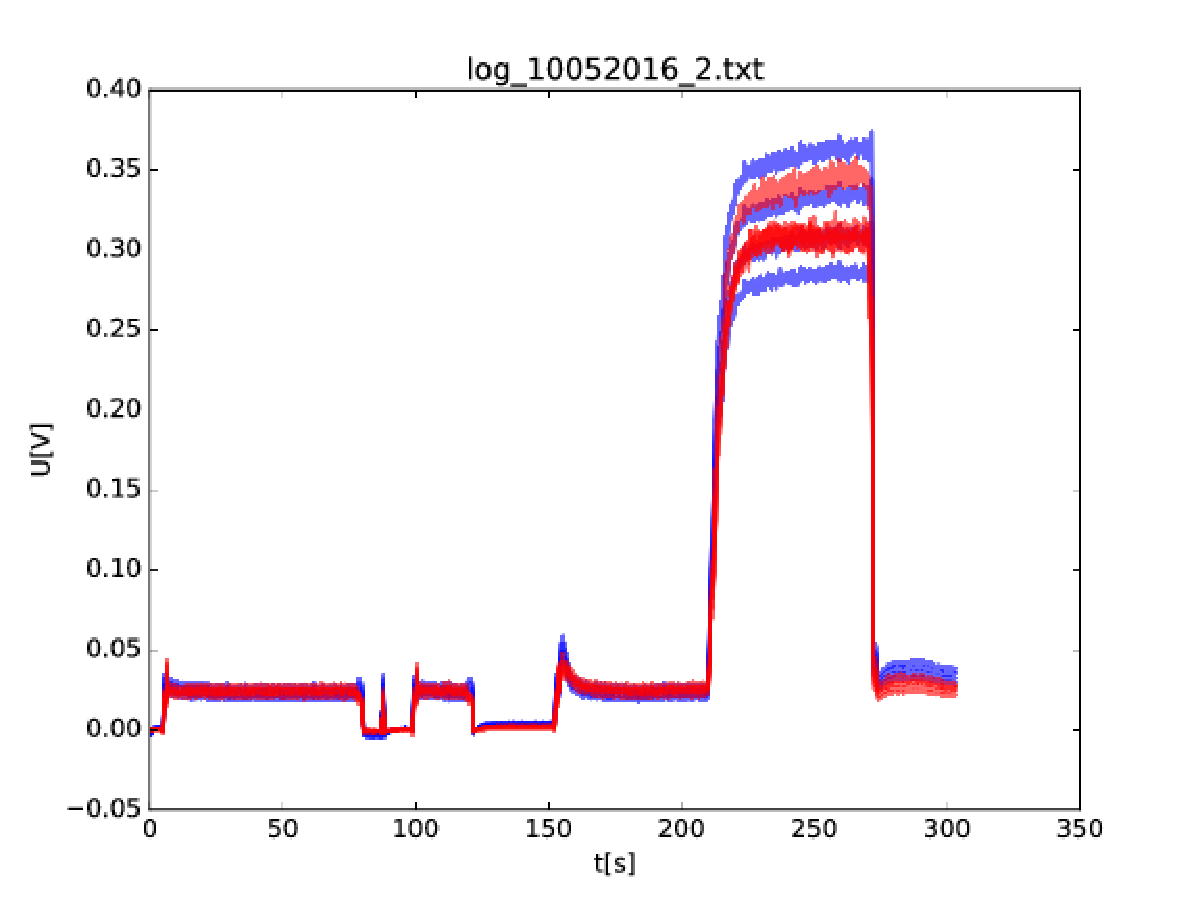
\includegraphics[width=\textwidth]{images/feed_switch.pdf} 
		\caption{feed switch}
	\end{center}
\end{figure}

\begin{figure}
	\begin{center}
		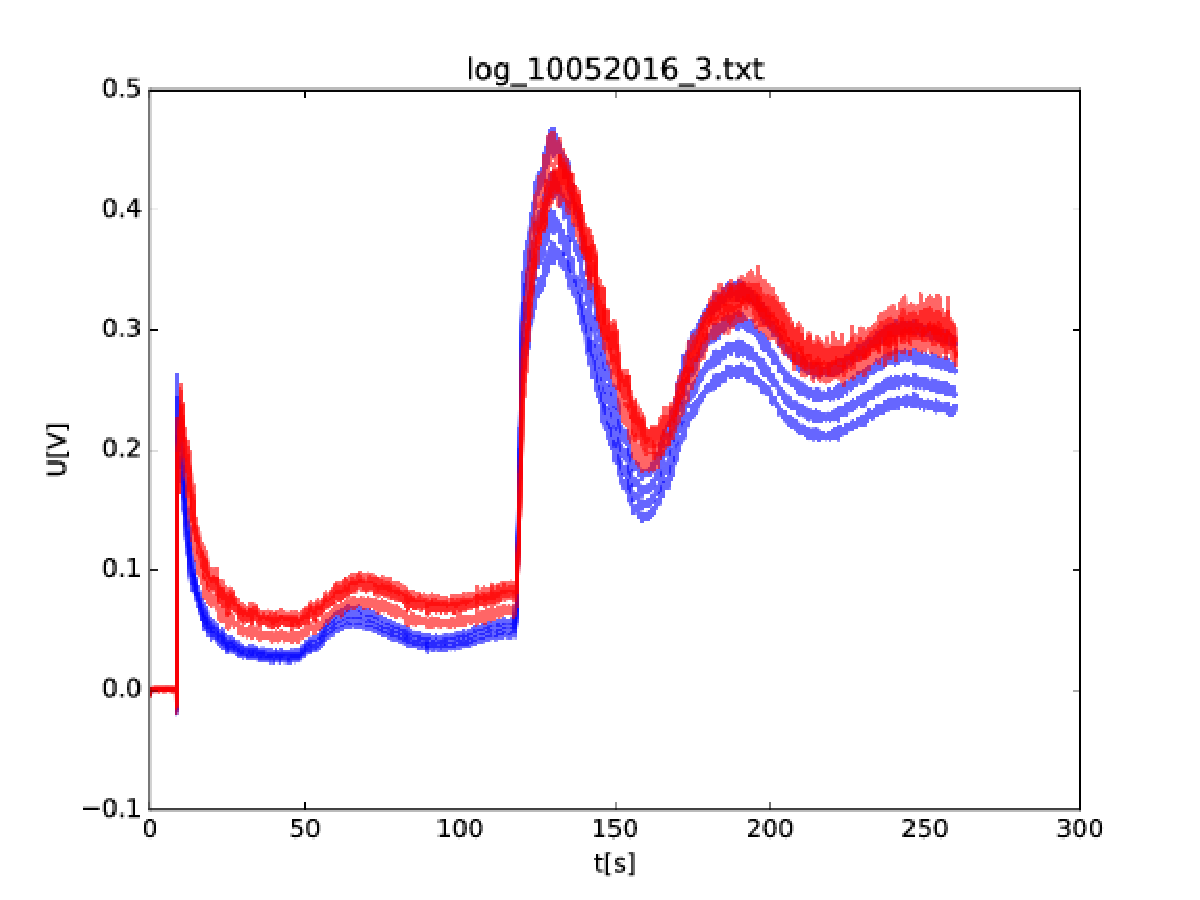
\includegraphics[width=\textwidth]{images/feed_add.pdf} 
		\caption{feed add}
	\end{center}
\end{figure}




\chapter{Conclusion}

The conclusion is it works.

%\chapter{Examples}

% Examples for tables. 
%   Note that second-level includes need to be done via \input{..},
%   since \include can not be nested
\section{Tables}

Tabelle \ref{tab:example} zeigt beispielhaft das Aussehen einer Tabelle in wissenschaftlichen Arbeiten. Überhalb der Tabelle ist eine horizontale Linie mittels \verb+\toprule+, unterhalb \verb+\bottomrule+. Mitten in der Tabelle können Abtrennungen mit \verb+midrule+ eingefügt werden, sollten zusätzliche Abtrennungen nötig sein. \\[\baselineskip]
Die Tabellenüberschrift ist im Gegensatz zu Bildern oberhalb der Tabelle zu finden. Fußnoten, welche in der Tabelle genutzt werden, können unterhalb der Überschrift oder unterhalb der Tabelle detailliert werden, sollten aber mit der Tabelle verknüpft sein und nicht erst am Ende der Seite zu finden.

\begin{table}[H]%
    \centering

    \caption[Beispieltabelle]{Beispieltabelle für den Aufbau
                von Tabellen in wissenschaftlichen Arbeiten.}
    \label{tab:example}
    \begin{tabular}{lcr}
        \toprule
        & Versuch 1 & Versuch 2 \tabularnewline
        \midrule
        Reaktor & \multicolumn{2}{c}{Photobioreaktor} \tabularnewline
        Algen & \textit{N. salina} & \textit{S. quadricauda} \tabularnewline
        \midrule
        $\mu_{max}$ & 0.3 & 0.25 \tabularnewline
        $K_m$ & 0.002 & 0.003 \tabularnewline
        \bottomrule
    \end{tabular}
\end{table}

Im folgenden ist der zur Tabelle gehörige Latex Code dargestellt:

\begin{Verbatim}[fontsize=\small,gobble=4]
    \begin{table}[H]%
        \centering

        \caption[Beispieltabelle]{Beispieltabelle für den Aufbau 
                    von Tabellen in wissenschaftlichen Arbeiten.}
        \label{tab:example}
        \begin{tabular}{lcr}
            \toprule
                & Versuch 1 & Versuch 2 \tabularnewline
            \midrule
            Reaktor & \multicolumn{2}{c}{Photobioreaktor} \tabularnewline
            Algen & \textit{N. salina} & \textit{S. quadricauda} \tabularnewline
            \midrule
            $\mu_{max}$, \unitfrac{1}{h} & 0.3 & 0.25 \tabularnewline
            $K_m$, \unitfrac{g}{l} & 0.002 & 0.003 \tabularnewline
            \bottomrule
        \end{tabular}
    \end{table}
\end{Verbatim}

Das \verb+[H]+ hinter der \verb+table+ Umgebung sorgt hierbei für die Platzierung der Tabelle an exakt dieser Stelle. Es kann weggelassen werden, hierbei verschieben sich die Tabellen aber teilweise beträchtlich. Weitere Infos findet man über die Internetsuche nach der Positionierung von "`Floating environments"'.

Die \verb+caption+ ist wie beschrieben vor der Tabelle und beinhaltet zwei Elemente, wovon das erste, optionale, (hier \verb+[Beispieltabelle]+) der Text ist, welcher in der Tabellenübersicht (\verb+\listoftables+) auftaucht. Damit kann und sollte man lange Tabellentitel für diese Übersicht kürzen. Für kurze Titel ist diese zusätzliche Angabe nicht erforderlich.

Das \verb+\label+ ermöglicht das Referenzieren (\verb+\ref+) der Tabelle, der hier hinterlegte Eintrag beginnt im Normalfall bei Tabellen mit \verb+tab:+ gefolgt von einem eindeutigen Namen. Mit diesem Namen kann die Tabelle im Text angesprochen werden (siehe Tabelle \ref{tab:example}).

Der Aufbau der Tabelle selber ist vergleichsweise komplex. Eine gute Übersicht bietet \url{http://en.wikibooks.org/wiki/LaTeX/Tables}. Für viele Anwendungen ist hier die Standardtabelle \verb+tabular+ ausreichend, besonders lange Tabellen können mittels \verb+longtable+ realisiert werden. Das empfohlene \verb+tabu+-Paket ist leider derzeit noch recht schlecht beschrieben, weswegen ich es (persönliche Meinung) leider nicht empfehlen kann.

\section{Graphen}

Graphen können in Latex direkt mit Hilfe der Pakete \verb+tikz+ und \verb+pgfplots+ (\url{http://www.ctan.org/pkg/pgfplots}) gemacht werden. Wie diese auszusehen haben ist dabei nicht so universell definiert wie bei den Tabellen. In Bild \ref{fig:example-graph} ist ein Beispiel für einen Plot dargestellt, wie er hier am Lehrstuhl gewünscht wird.

\begin{figure}[H]%
    \centering
    % do not externalise this picture
    \tikzset{external/export next=false}
    
    \begin{tikzpicture}
        \begin{axis}[
            ymin=-1.5, ymax=1.5,
            xmin=0, xmax=15,
            width=15cm, height=10cm,
            ylabel={Speed, \unitfrac{m}{s}},
            xlabel={Time, \unit{s}},
            ignore legend
            ]
        
            \addplot+[only marks, mark=x, mark size=3, forget plot] table[x=time, y=value, col sep=semicolon] {data/measurements-data.csv};
            \addlegendentry{Messdaten Sinus}
            \label{graph:measurement-sine}
            \addplot+[mark=none] table[x=time, y=value, col sep=semicolon] {data/simulation-data.csv};
            \addlegendentry{Simulationsdaten Sinus}
            \label{graph:simulation-sine}
            
            \addplot+[simulation-plot] plot[domain=0:15, samples=500, smooth] {cos(x/pi*180)}; 
            \label{graph:simulation-cosine}
        \end{axis}
    \end{tikzpicture}
    
    
    \caption{Beispielgraph. Dargestellt sind die Messdaten der Sinuskurve (\protect\plotref{graph:measurement-sine}), die zugehörige Simulation (\protect\plotref{graph:simulation-sine}) sowie eine Simulation, die eine Alternative konfiguration wiedergibt (\protect\plotref{graph:simulation-cosine})}%
    \label{fig:example-graph}%
\end{figure}

Generell haben Graphen in schriftlichen Arbeiten keinen Titel. Achsenbeschriftungen sind zwingend erforderlich (vgl. Abbildung \ref{fig:label-your-axes-xkcd}) und müssen mit einer Einheit versehen werden. Die Beschriftung der Achsen und der Zahlen sollte nicht zu klein sein (Schriftgröße mind. 14pt, in latex \verb+\normalsize+).

\begin{figure}[H]%
    \centering

    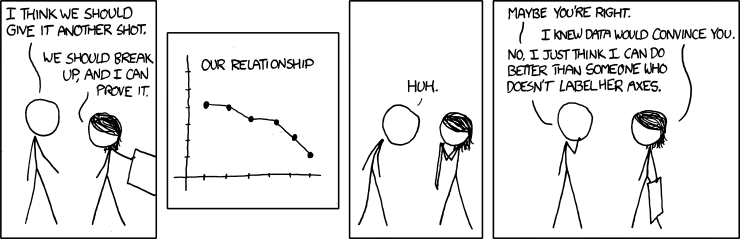
\includegraphics[width=0.8\columnwidth]{images/examples/axes-xkcd}%
    \caption{"`Convincing"', \href{http://xkcd.com/833/}{xkcd.com/833}}%
    \label{fig:label-your-axes-xkcd}%
\end{figure}

Weiterhin gilt:

\begin{itemize}
	\item Um den Graph herum ist ein schwarzer, ertwas dickerer Rahmen zu ziehen (Latex/pgfplots: \verb+axis line style={thick}+).
    \item Hilflinien sind in dünn und hell bei den Hauptachsenmarkierungen waagrecht und senkrecht zu zeichnen. Die Linien können dabei durchgezogen oder gestrichelt sein. In Latex/Pgfplots wird das gezeigte Ergebnis durch \verb+grid=major+ und \verb+grid style={help lines, dashed, thin}+ erreicht.
    \item Messwerte werden durch einzelne Markierungen dargestellt, während simulierte Daten durchgängige Linien erhalten. Die Farben sollten so gewählt werden, dass der Ausdruck in schwarz/weiss erkennbar ist. Zusammengehörige Mess-/Simulationsdaten können dabei die gleiche Farbe erhalten. Für Messdaten kann die s/w--Eindeutigkeit durch Wechsel des Symbols erleichtert werden.
    \item Am Lehrstuhl wird die Legende nicht im Graph dargestellt, sondern in der Bildunterschrift. Dies kann bei pgfplots über das setzen von \verb+\label+s und Referenezierung über \verb+\protect\ref+ erreicht werden. \textcolor[rgb]{0.55,0,0}{Achtung}: Bei Nutzung von \verb+\tikzexternalize+ kann dies zu Fehlern führen! Hierbei muss die Externalisierung für die Refernez deaktiviert werden. Dazu kann auch das in dieser Vorlage definierte \verb+\plotref+ genutzt werden.
\end{itemize}

Vereinfacht können die generellen Darstellungseigenschaften eines Graphen über den folgenden Eintrag in der Präambel des Dokuments definiert werden, wie es in dieser Vorlage (\verb+elements/preamble.options.tex+) bereits umgesetzt ist:

\begin{Verbatim}[fontsize=\small,gobble=4]
    \pgfplotsset{
        every axis/.append style={
            grid=major,
            grid style={help lines, dashed, thin},
            axis line style={thick},
            title style={font=\large\bfseries, text centered},
            label style={font=\normalsize},
            tick label style={font=\normalsize},
        }
    }
\end{Verbatim}

Um die Darstellung der Simuations- und Messdaten zu vereinfachen, existieren in dieser Vorlage weiterhin Kürzel, welche bei Plots genutzt werden können um die generelle Darstellung zu vereinfachen (\verb+elements/preamble.tweaks.tex+). Für eine genaue Bedeutung der jeweiligen Befehle möchte ich auf das \href{http://mirrors.ctan.org/graphics/pgf/contrib/pgfplots/doc/pgfplots.pdf}{pgfplots-Manual} verweisen. Ein Beispiel für de Anwendung findet sich im Code von Graph \ref{fig:example-graph}. 

\begin{Verbatim}[fontsize=\small,gobble=4]
    \pgfplotsset{
        simulation-plot/.style = {
          each nth point=10, filter discard warning=false,
          mark=none, 
          x=Time,
          thick,
          },
        measurements-plot/.style = {
          mark=*, only marks, mark size=2pt, mark options={},
          x=Time,
          forget plot,
          error bars/y dir=both, error bars/y fixed relative=0.05,
          },
    }
\end{Verbatim}

Und --- last but not least --- nochmal der Hinweis:

\begin{figure}[H]%
    \centering
    
    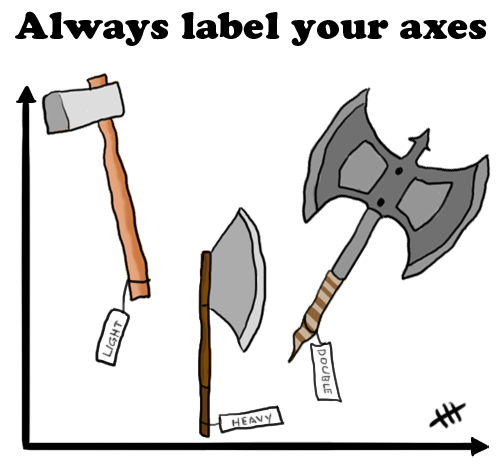
\includegraphics[width=0.4\columnwidth]{images/examples/axes-fluffware}%
    \caption{"`Always label your axes"', Quelle \href{http://fluffware.tumblr.com/post/4580822773/axes}{Fluffware}}%
    \label{fig:label-your-axes-fluffware}%
\end{figure}


\section{Images}

In Planung


%% Appendix
\appendix
\chapter*{Appendix}                         % Appendix headline
\addcontentsline{toc}{chapter}{Appendix}    %   and entry in Table of Contents

% Abbreviations chapter
\chapter{Abbreviations}

{
% Force full \textwidth
\setlength\LTleft{0pt}
\setlength\LTright{0pt}

\begin{longtable}{p{3cm}l@{\extracolsep{\fill}}}
    CFD   & Computational Fluid Dynamics \tabularnewline
    PBR   & Photobioreactor \tabularnewline
    PC & Personal Computer \tabularnewline
    I2C & Inter-Integrated Circuit \tabularnewline
    SPI & Serial Peripheral Interface \tabularnewline
	GND & electrical ground \tabularnewline
    SIG & Signal \tabularnewline
    PCB   & Printed Circuit Board \tabularnewline
    flex-PCB   & flexible Printed Circuit Board \tabularnewline
    opamp  & Operational Amplifier \tabularnewline
    OUT & Output \tabularnewline
    SCLK & Clock Signal \tabularnewline
    DIN & Digital Input \tabularnewline
    DOUT & Digital Output \tabularnewline
    D & Drain \tabularnewline
    S & Signal \tabularnewline
    SYNC & Synchronization \tabularnewline
    ADC & Analog-Digital-Converter \tabularnewline
    AC & Alternating Current \tabularnewline
	GUI & Graphical User Interface \tabularnewline
	Command Line Interface & (CLI) \tabularnewline
\end{longtable}
}

% Have list of figurs and tables on the same page, uncomment weird stuff to have them seperate again
\listoffigures
\begingroup
\let\clearpage\relax
\listoftables
\endgroup

% Bibliography

\printbibliography

\end{document}
